\documentclass[
    %draft, % Mit % kommentieren, um Bilder sichtbar zu machen und Links zu aktivieren
    pdftex,
    a4paper,
    twoside,
    parskip=half,
    numbers=noenddot,
    listof=totoc,
    bibliography=totoc,
    hyperfootnotes=false,
    english,
    openright
]{scrreprt}

% FIXME: this doesn't work: https://blog.rtwilson.com/how-to-add-simple-new-commands-to-latex-to-help-with-writing-papers/ (11.04.2025)
\newcommand{\todo}[1] {\textbf{\textcolor{red}{TODO:}} #1}
\newcommand{\thesistitle}{\todo}
\newcommand{\thesistype}{M A S T E R \space \space T H E S I S}
\newcommand{\thesistypedesc}{Department of Electrical Engineering and Computer Science \\
    University of Kassel}
\newcommand{\thesisauthorname}{Klara Maximiliane Gutekunst}
\newcommand{\thesisauthorhomestreet}{\todo}
\newcommand{\thesisauthorhometown}{34119 Kassel}
\newcommand{\thesisauthormatrikelnumber}{35677772}
\newcommand{\thesisauthoremail}{klara.gutekunst@uni-kassel.de}
\newcommand{\thesisdepartment}{Chair Deep Semantic Learning}
\newcommand{\thesisfirstreviewer}{Prof.\ Dr.\ Martin Potthast}
\newcommand{\thesissecondreviewer}{Prof.\ Dr.\ Gerd Stumme}
\newcommand{\thesissupervisor}{\todo}
\newcommand{\thesisdate}{\today}

% content-specific commands
\newcommand{\tira}{TIRA}

% Select input encoding, usually utf8 is the best choice, on windows, \usepackage[latin1]{inputenc} maybe required
\usepackage[utf8]{inputenc}
\usepackage[T1]{fontenc}
\usepackage[english]{babel}
\usepackage{csquotes}
\usepackage{xcolor}

\MakeOuterQuote{"} % Damit ist es möglich, " " zu verwenden ohne Umlaut zu erzeugen
\defaulthyphenchar=127 % Dadurch werden auch Wörter mit Bindestrich getrennt, die schon Bindestriche enthalten.

% geometry
\usepackage[bindingoffset=1cm, left=2.5cm, right=2.5cm, top=2.5cm, bottom=2.5cm]{geometry}

% Headline
\usepackage{fancyhdr}
\pagestyle{fancy}
\renewcommand{\chaptermark}[1]{\markboth{\thechapter\ #1}{}}
\lhead{\leftmark} \rhead{\thepage}
\cfoot{}
\fancypagestyle{plain}{}

\RedeclareSectionCommand[beforeskip=1.5cm,afterskip=1cm]{chapter}

% Colors
\usepackage{color}
\usepackage{colortbl}

% Tables
\usepackage{tabularx}
\usepackage{multirow}
\setlength{\tabcolsep}{4pt}

% Drawing graphs etc.
\usepackage{pgf}
\usepackage{tikz}
\usetikzlibrary{arrows,automata}

% Footnotes
\usepackage{footmisc}
\usepackage{xspace}
\newcommand{\sic}{[\acs{sic}]\xspace}

% math
\usepackage{amsmath}
\usepackage{amssymb}

\usepackage{siunitx}

% lists
\usepackage{paralist}

% Figures
\usepackage{graphicx, wrapfig}

% Hyperlinks
\usepackage[hyphens]{url}
\usepackage{hyperref}
\hypersetup{colorlinks, citecolor=black, linkcolor=black, urlcolor=black}

% Minted
\usepackage[chapter]{minted}
%\usemintedstyle{xcode}
\setminted{frame=single,tabsize=2,linenos,autogobble}

\newmintinline[code]{text}{breaklines}

\newminted[mdcodeblock]{md}{autogobble,frame=none,linenos=false,breaklines}

% list of abbreviations
\usepackage[printonlyused]{acronym}

% Set line pitch
\usepackage{setspace}
\onehalfspacing              % anderthalbzeilig (oder auch \doublespace)

%fancyBox
%\usepackage{fancybox}

% Layout corrections (Schusterjungen)
\clubpenalty = 10000
% Layout corrections (Hurenkinder)
\widowpenalty = 10000
\displaywidowpenalty = 10000

% Figures
\usepackage{caption}
\usepackage[hypcap=true,labelformat=simple]{subcaption}
\renewcommand{\thesubfigure}{(\alph{subfigure})}
\usepackage[inkscapelatex=false]{svg}

% Tables
\usepackage{booktabs}
%\usepackage[table,xcdraw]{xcolor}

% enumerate
\usepackage{enumitem}
\newlist{questions}{enumerate}{2}
\setlist[questions,1]{label=RQ\arabic*.,ref=RQ\arabic*}
\setlist{nolistsep}

% Bibliography
\usepackage[square,numbers]{natbib}
\bibliographystyle{plainnat} % or plainnat abbrvnat unsrtnat

% Frequently used column types
\newcolumntype{C}[1]{>{\centering\arraybackslash}p{#1}} % centering column type with fixed width
\newcolumntype{R}[1]{>{\raggedleft\arraybackslash}p{#1}} % right aligned column type with fixed width
\newcolumntype{L}[1]{>{\raggedright\arraybackslash}p{#1}} % left aligned column type with fixed width

% Shortcuts for referencing floats:
\newcommand{\fig}[1]{\figurename~\ref{#1}} %shortcut for a figure reference
\newcommand{\tab}[1]{Table~\ref{#1}} %shortcut for a table reference
\newcommand{\eq}[1]{(\ref{#1})} %shortcut for an equation reference
\newcommand{\lst}[1]{Listing~\ref{#1}} %shortcut for a listing reference
\newcommand{\sect}[1]{Section~\ref{#1}} %shortcut for a Section reference
\addto\extrasenglish{%
  \renewcommand{\sectionautorefname}{Section}%
  \renewcommand{\subsectionautorefname}{Subsection}%
  \renewcommand{\chapterautorefname}{Chapter}%
}

% Shortcut for terms
\newcommand{\databaseName}{Elasticsearch}
\newcommand{\flask}{Flask}
\newcommand{\angular}{Angular}
\newcommand{\infersent}{InferSent}
\newcommand{\wordcloud}{word cloud}
\newcommand{\localMaschineStats}{Apple M2 Pro MNW83D/A with 16 \ac{gb} RAM and 12 cores}
\newcommand{\slurm}{Slurm}




\begin{document}
    \pagenumbering{roman}

    % \include{titlepage}
    % \chapter*{Abstract}
\markboth{Abstract}{Abstract}

\Acl{av} seeks to determine whether two texts share the same author, a task critical for ensuring the integrity of academic submissions or online content.
Existing approaches typically exhibit poor generalisation across domains.
The \impAppr{} introduced hard negative sampling to create input-pair-specific settings to improve cross-domain generalisation. 
However, traditional sampling strategies are unable to simultaneously control for multiple confounding variables, such as genre and topic.
%, highlighting the need for improved sampling strategies.
This thesis investigates whether \aclp{llm} can help address these limitations. 
Specifically, we employ \acs{llm}-generated paraphrases as hard negatives. 
% Since these paraphrases aim to preserve the confounding variables of the original text, they mitigate domain-related biases during inference. 
% Moreover, by constructing a tailored case for each input text pair, the approach eliminates out-of-distribution issues, ensuring that comparisons remain within the distribution defined by the pair itself.
Evaluation on the \dataStudent{} dataset from the original study shows that the \acs{llm}-based extension surpasses the original baselines by \citet{koppel_determining_2014}, \acs{ppmd}, and \unmasking{} in terms of precision and recall.
At the same time, our results reveal the practical and conceptual challenges of integrating \acsp{llm} into \acl{av}, including issues of reliability, hallucination, and control over paraphrase quality.



% The original \impAppr{} compares a disputed text to a candidate text and hard negatives, considering disputed and candidate text to share an author if the candidate is consistently the most similar across random feature projections. 
    % \chapter*{Zusammenfassung}
\markboth{Zusammenfassung}{Zusammenfassung}



    % \tableofcontents

    \chapter*{List of abbreviations}
\markboth{List of abbreviations}{List of abbreviations}

\begin{acronym}[XXXXXXXXX]
    \acro{ai}[AI]{Artificial Intelligence}
    \acro{ir}[IR]{Information Retrieval}
    \acro{nlp}[NLP]{Natural Language Processing}
    \acro{llm}[LLM]{Large Language Model}
    \acro{roc-auc}[ROC-AUC]{Area Under the Receiver Operating Characteristic Curve}
    \acro{pan}[PAN]{Plagiarism Analysis and Authorship Mining} % TODO: find out if correct
    \acro{bert}[BERT]{Bidirectional Encoder Representations from Transformers}
    \acro{bow}[BoW]{Bag-of-Words}

    % \acro{}[]{}
\end{acronym}


    % \pagebreak
    \pagenumbering{arabic}

    % % Hier weitere Kapitel einfügen
    \chapter{Introduction}
\label{chap:introduction}



% motivation
Historically, authorship analysis focused on literary disputes~\citep{neal_surveying_2018,stamatatos_survey_2009}, but contemporary concerns have shifted towards practical applications.
In an era where large amounts of text can be copied, paraphrased, or fabricated with ease, determining the true author of a text is crucial for maintaining trust in communication. 
Scenarios include detecting plagiarised passages of texts~\citep{stein_intrinsic_2011}, and verifying the authenticity of online content or student submissions. 
Formally, we refer to these problems as \acf{av} or \acf{aa}, where every \ac{aa} task can be formulated as a sequence of \ac{av} problems~\citep{tyo_state_2022,barlas_cross_domain_2020}.

The emergence of \acp{llm} adds an additional layer of complexity. 
While these models are widely embraced for beneficial applications such as summarisation, information seeking, and assistive writing~\citep{wang_stumbling_2024}, their ability to convincingly imitate human writing creates new risks. 
\acp{llm} can be used to generate misinformation, impair academic honesty, or impersonate individuals, thereby inflicting harm on individuals who fall victim to these schemes~\citep{mitchell_detectgpt_2023,li_learning_2025,wang_stumbling_2024,bhattacharjee_fighting_2024}. 
Since \acp{llm} can be conceptualised as authors, their detection naturally falls within the scope of \ac{av}. 
Thus, instead of treating \ac{llm} detection as an isolated task, it is more consistent to frame it as a specialised case of \ac{av}~\citep{llm_detection_av_2025}.

% specificity rather than generality
Existing approaches to generalisation typically train a single model and apply it across domains.
Despite significant advances in \ac{av}, prior work finds that such models struggle in \ac{ood} settings, where the topic or genre diverges from the training data~\citep{Sundararajan_style_18,bischoff_importance_2020,li_learning_2025}. 
This shortcoming motivates a shift towards scenario-specific solutions, i.e.\ models are trained anew for narrowly defined cases. 
Such single-case approaches enable more precise control over contextual factors and place greater emphasis on stylistic idiosyncrasies rather than domain-level variation.

% AV
The \impAppr{} by \citet{koppel_determining_2014}\ introduces the idea of generating \imp{} texts, i.e.\ hard negatives, used to sharpen the discrimination between genuine and false authorship matches. 
However, the method's effectiveness is limited by the quality and contextual adequacy of these \imp{} texts. 
Previous work did not fully address how to construct challenging \imps{} via controlled contextual variables.

The thesis extends the \impAppr{} by leveraging \acl{sota} \acp{llm} to generate paraphrases as \imps{}, enabling control over multiple confounding factors such as genre, topic, and target audience. 
In doing so, the approach shifts the focus towards authorial style rather than domain differences, yielding improved precision–recall on the \dataStudent{} dataset compared with the original sampling strategies, \unmasking{} and \acs{ppmd}.


\section{Research Questions}
\label{sec:research_questions}
To guide this objective, we formulate the following research questions:
\begin{questions}
    \item \textbf{How can we instruct a \ac{llm} to paraphrase the text of a candidate author such that it captures the \ac{llm}'s stylistic properties?} \label{enum:rq1} \hfill \\
    The goal is to create hard negatives for the Impostor method by controlling contextual factors.
    By controlling genre, topic and other factors, similarity measures primarily focus on differences in authorial style rather than the impact of content on style.
    We obtain this controlled environment by utilizing \acp{llm} to paraphrase the original text.
    There are different approaches to paraphrasing text using \acp{llm}.
    They include (a) directly asking the \ac{llm} to paraphrase the text, 
    (b) first extracting specific information from the original text and subsequently generating a paraphrase based on the information.
    This thesis compares both approaches on \dataStudent{}, \dataBlog{}, \dataGutenberg{} and \dataPan{}.

    \item \textbf{How do we evaluate the quality of paraphrases?} \label{enum:rq2} \hfill \\
    Paraphrase evaluation is inherently challenging, as there is no universally agreed-upon definition of what constitutes a paraphrase. 
    Prior research often adapts evaluation metrics from related \ac{nlp} tasks such as machine translation or summarization. 
    Two key dimensions are typically considered: semantic similarity and syntactic similarity.
    Contrary to initial intuition, high syntactic similarity is not necessarily desirable, as it may indicate that the \ac{llm} has merely copied the original text with minimal changes. 
    Instead, our focus lies on achieving high semantic similarity while maintaining syntactic diversity to ensure genuine rephrasing.
    Furthermore, we acknowledge that relatively low automatic scores can still be acceptable if qualitative human evaluation confirms the paraphrase’s adequacy.

    % \item \textbf{Which features are used for the \ac{av} problem?} \label{enum:rq3} \hfill \\
    % Traditional features include character tri-gram features, while newer research has proposed using \ac{llm} such as BERT.

    \item \textbf{How does the \ac{llm}-based impostor approach perform compared to state-of-the-art models?} \label{enum:rq4} \hfill \\
    Though our approach is computationally expensive, we argue that it is not a general purpose \ac{llm} detection method, but rather a single case solution tailored to specific detection tasks.
    We evaluate its performance in scenarios where (a) the disputed text is human generated,
    (b) the disputed text is \ac{llm} generated and the candidate is the same \ac{llm}, and
    (c) the disputed text is \ac{llm} generated, but the candidate is a different \ac{llm}.
    In terms of performance, we compare our method to other \ac{av} approaches on the \dataStudent{}, \dataBlog{}, \dataGutenberg{} and \dataPan{} datasets.
    
\end{questions}

% \section*{Idea}
% \label{sec:idea}

% Given a text of unknown authorship (i.e., human or \ac{llm}), 
% construct a set of impostor texts using state-of-the-art \acp{llm} based on the original text.
% Obtain the author by \ac{aa}/ \ac{av} methods, such as unmasking, to \textit{confidently}, i.e. high precision, identify \ac{llm} generated texts
% (and possibly which \ac{llm}).



\section{Contributions}
\label{sec:contributions}
The contributions of this thesis are:
\begin{enumerate}
    \item Reimplementation of the traditional Impostor approach (cf. \autoref{chap:implementation}).
    \item Extension of the impostor approach with \ac{llm} generated impostors for line-up of difficult opponents (cf. \autoref{chap:methodology}). 
    \item Frame \ac{llm} detection as a \ac{av} problem and use \ac{llm} generated text as candidate for text of "unknown" authorship.
\end{enumerate}


\section{Thesis Structure}
\label{sec:thesis_structure}
The thesis is structured as follows:
    \chapter{Related Work}
\label{chap:related_work}

This work is different to the work of \citet{koppel_determining_2014} and \citet{kocher_unine_2015} 
in that it uses \acp{llm} to generate imposter texts.

% AV

% LLM detection using generative models
%% AA against LLMs
With the recent advances of \ac{nlg} come new challenges in text authorship.
The new technologies may be misused for fraudulent activities to scam naive or inexperienced users~\citep{uchendu_authorship_2020,bhattacharjee_fighting_2024}.
\citet{uchendu_authorship_2020} identified three authorship tasks essential for fighting fraudulent activities:
(1) Given two texts $t_1$ and $t_2$, determine whether they were produced by the same method (i.e. human author or a specific \ac{nlg} method).
(2) Given a text $t$, determine whether it was human authored or machine generated (Turing Test).
(3) Given a text $t$, find its author among $k+1$ candidates, which consists of one human and $k$ machines.
They compare classical \ac{ml} models, neural models and state-of-the-art \ac{aa} models as classifiers 
for these single- (Problem 1 and 2) and multi-class (Problem 3) tasks.
Their findings include, that as of 2020, most \ac{nlg} methods were distinguishable from human authors, 
but some \acp{llm} proved difficult to detect.
%%% compared to our work
In the following, we consider (1) \ac{av}, (2) classical \ac{llm} detection, and (3) closed-set \ac{aa}.
Our approach differs from the work of \citet{uchendu_authorship_2020} in that our candidates (i.e. imposters) do not include a human author (3), 
but only \acp{llm}.
Moreover, we use different classifiers originally designed for \ac{av}, rather than \ac{aa}.

%% LLM (gpt-3.5, GPT-4) as detector
\citet{bhattacharjee_fighting_2024} evaluate using an \ac{llm} as classifier for \ac{llm} detection.
They use \ac{gpt}-3.5 and \ac{gpt}-4 to classify texts as human or machine generated.
They find that \ac{gpt}-3.5 performs better when being fed simple instructions, rather than constrained prompts.
They find that \ac{gpt}-4 predicts almost exclusively \ac{ai} generated texts, 
while \ac{gpt}-3.5 predictions are more reliable (especially for actually human authored texts).
%%% compared to our work
Our work differs from theirs in that we use \acp{llm} to generate imposter texts specific to the candidate text, 
rather than using the publicly available dataset TuringBench with previously generated texts.

%% DetectGPT: Perturb (Mask), score, compare (unsupervised)
\citet{mitchell_detectgpt_2023} propose DetectGPT, a method that is threefold:
(1) They perturb the input text by (1.1) masking out random 2-word spans until 15 \% of the text is masked. 
Masked spans are replaced (1.2) with words from an off-the-shelf (i.e. not finetuned to target domain) \ac{llm} (e.g. T5-3B). 
These perturbations are semantically similar paraphrases of the original text.
(2) They score (in terms of log probability) each perturbed text using a scoring \ac{llm} 
(ideally their candidate \ac{llm}, but it works also with any \ac{llm}, though scores deteriorate). 
(3) The difference of the score of the original text and the average score of the perturbed texts is denoted perturbation discrepancy $d$. 
(4) Normalize $d$ by the standard deviation of the scores of the perturbed texts.
(5) Based on a threshold $\epsilon=0.1$, classify the original text as human authored or machine generated 
(formally Local Perturbation Discrepancy Gap hypothesis).
If $d$ is positive, the original text is likely machine generated.
If $d$ is near zero, i.e. $d < \epsilon$, the original text is likely human authored.
\citet{mitchell_detectgpt_2023} motivate their method by the observation that generated texts tend to occupy 
negative curvature regions of the model's log probability function (i.e. they lie on the local maximum of the manifold).
When the text is machine generated, it lies on a local maximum, 
and perturbing it will lead to lower log probabilities of perturbed texts.
When the text is human authored, it does not lie on a local maximum to begin with, 
rendering log probabilities of perturbed texts similar either bigger or smaller than the original text.
Averaging the log probabilities of perturbed human texts leads to a value that is 
close to the original text's log probability (i.e. a perturbation discrepancy $d$ near zero).
Even though, DetectGPT works best when the source (i.e. generating) \ac{llm} and the scoring \ac{llm} are the same 
(requires white-box access to the \ac{llm}), 
it works also with different \acp{llm} as surrogate for the source model when scoring (in a black-box case).
%%% compared to our work
We can not supply a white box setting, because we do know the source \ac{llm} that generated the imposter texts.
%%%% imposters and perturbations
However, this approach is similar to our approach, because perturbing texts can be seen as a 
form of imposter generation (especially as we use paraphrases). 
%%%% sample from the source model
Both approaches try to sample from the probability distribution of the source model either 
by using imposters (via prompting an \ac{llm}) or by perturbing the original text (using an \ac{llm}).
%%%% input
While the imposter approach is an \ac{av} task (i.e. input is a disputed and a candidate text), 
DetectGPT receives a disputed text and a candidate \ac{llm} as input.
%%%% similarity measure
While we use a similarity measure on traditional n-gram frequency vectors, 
\citet{mitchell_detectgpt_2023} require a scoring \ac{llm} to compute the perturbation discrepancy $d$.
Hence, our approach is easier in terms of computational resources and requirements.

%% LLM rewrite LLM texts less than human texts (no AA, but edit distance hypothesis)
RAIDAR~\citep{mao_raidar_2024} builds upon the invariance property of \acp{llm}, 
which states that prompting an \ac{llm} to rewrite a machine generated text will introduce little change.
They motivate this by the observation that (different) autoregressive models produce similar patterns and thus, 
consider texts generated by (different) \acp{llm} as high quality that do not require rewriting.
Change is measured by the edit distance between the original text and the rewritten text. 
\citet{mao_raidar_2024} propose using an edit distance based on the Levenshtein distance or \ac{bow} representations.
RAIDAR operates on character level rather than using deep neural network features, and it does not require the original generating model for classification. 
RAIDAR fails to detect \ac{llm} generated texts in out-of-distribution scenarios (i.e. different domains than training), 
or when \ac{llm} were explicitly instructed to produce text prone to heavy \ac{llm} modification when being asked to rewrite the text \citep{li_learning_2025}.
Based on RAIDAR (\citep{mao_raidar_2024}), \citet{li_learning_2025} propose fine-tuning an \ac{llm} to rewrite human authored texts more than machine generated text.
Classification is carried out by comparing the edit distance of the original text and the rewritten text to a threshold.
\citet{li_learning_2025} admit that their approach is slow in inference time, 
since a candidate text has to be rewritten multiple times (about 200 different prompts) to obtain a reliable score.
\citet{mao_raidar_2024} find that the quality of perturbation based models (i.e. rewriting) for \ac{llm} detection correlates with the perturbation model size.
\citet{mitchell_detectgpt_2023} find a negative correlation (\textcolor{red}{TODO: chapter 2 vorletzter Absatz}) between the size of the perturbation model and the performance of DetectGPT.
%%% compared to our work
%%%% generation of texts during inference
Both approaches are similar to our work in that they use \acp{llm} to generate texts during inference.
We do not fine-tune an \ac{llm} for paraphrasing but use off-the-shelf models (like RAIDAR).
%%%% similarity measure
All these approaches compute the similarity of the original text and the generated text.
However, we do not use edit distance (i.e. Levenshtein distance) as similarity measure.
%%%% limitations
This approach is unable to detect which \ac{llm} generated the text.

%% LLMDet: Proxy to perplexity (problem: requires access to the LLM to build the dictionary)
Perplexity is a reliable statistical metric for attributing texts to \acp{llm}~\citep{zhang_llmdet_2023}.
Unfortunately, perplexity requires access to \acp{llm}' parameters (i.e., white-box detection).
\citet{zhang_llmdet_2023} propose LLMDet, a method that uses a proxy to perplexity, 
where a dictionary of frequent n-gram (frequent among $n$ randomly prompted generated texts per \ac{llm}) 
next token probabilities is pre-computed (i.e. requiring access to the \ac{llm}), 
and is subsequently used during inference to approximate perplexity by replacing $x_{<i}$ in $p(x_i | x_{<i})$ with an n-gram.
Since the construction of the dictionary requires access to the \ac{llm}, LLMDet requires contribution of the closed-source model owners.
The disputed text is tokenized and the proxy perplexity is calculated for each model and thus, constructing a proxy perplexity vector.
This vector is input to a trained classifier.
%%% compared to our work
Proxy perplexity could be used as a baseline for our approach, though it requires access to the \ac{llm} and is thus not applicable in our case.

%% Mirror Minds: extract query, genrate two paraphrases, compare & classify via threshold (very similar to our work)
\citet{baradia_mirror_2025} propose (1) extracting a query from the disputed text, which captures the essence of the text, 
(2) generating two paraphrases of the original text using the query as input prompt to two \acp{llm}, 
and (3) comparing the paraphrases to the original text via the BLEU and the METEOR score.
Both score capture syntactic similarity, even though \citet{baradia_mirror_2025} argue they also capture semantic similarity.
They use the maximum across the two models per similarity measure as a final score pair.
Classification of the resemblance to \ac{ai} generated content requires a threshold.
%%% compared to our work
%%%% same approach
This approach is similar to our approach in that it uses \acp{llm} to generate paraphrases of the original text.
Moreover, it compares the original text to the generated paraphrases as in a \ac{aa} problem. % rather AI detection?????
%%%% similarity measure
We do not use BLEU or METEOR as similarity measure, nor do we compare directly on paraphrase-level (i.e. BLEU calculates n-gram overlap) 
but construct our own frequency based n-gram vectors input vector similarity metrics.
%%%% they discard information, solve another problem
However, this approach discards the information which \ac{llm} produced the most similar paraphrase. 
While our goal is to solve an \ac{aa} problem (i.e. multiclass classification), 
\citet{baradia_mirror_2025} solve a binary classification problem (i.e. human vs. \ac{ai} generated text).
    % \chapter{Methodology}
\label{chap:methodology}

\subsection{Dataset}
\label{subsec:dataset}

\subsubsection{Original Data}
Due to this approach extending the original imposter approach by \citet{koppel_determining_2014}, 
we first use original data to establish the feasibility and reproducibility of the original approach. 
\citet{koppel_determining_2014} used \dataBlog{} and the \dataStudent{} dataset.
The  \dataStudent{} dataset is not publicly available, due to sensible information about the students.
J. W. Pennebaker was kind enough to provide us with the original data M. Koppel used in his paper.
The dataset contains student essays for five assignments from a class in 2006.
The assignments include stream of consciousness, talk about your childhood, describe your personality, 
Thematic Apperception Test, and Give four examples of four different theories.
For reproducing our work, due to privacy concerns, 
we refer to J. W. Pennebaker as the data holder  and authority of the \dataStudent{} dataset.
For establishing a baseline for the imposter approach, we use the \dataBlog{} and the \dataStudent{} dataset.

\subsubsection{Additional Data}
To extend our test scenario for the imposter approach, we opted to find an additional dataset that fulfilled the following criteria:
\begin{itemize}
    \item controlled confounders (e.g. genre, topic)
    \item undisputed authorship 
    
\end{itemize}

We found that both the \dataPan{} and \dataGutenberg{} datasets are suitable candidates.
The statistical properties of the datasets are shown in \autoref{tab:data_stats}.

\begin{table}[h]
\centering\small
\caption{Statistics of preprocessed datasets \dataPan{}, \dataBlog{} and \dataGutenberg{}.}
\label{tab:data_stats}
\resizebox{\textwidth}{!}{%
\begin{tabular}{@{}lrrrrrrrrr@{}}   % numbers should be right aligned, text left aligned
\toprule
dataset & num\_pairs & num\_authors & num\_same\_pairs & num\_different\_pairs & avg\_text\_len & min\_text\_len & max\_text\_len & std\_text\_len & median\_text\_len \\ 
\midrule
pan20     & 66912 & 52778 & 35620 & 31292 & 21435.53  & 20670 & 296887  & 2685.49   & 21284.00  \\ 
blog      & 64771 & 18961 & 33639 & 31132 & 1846.20   & 501   & 615409  & 3461.74   & 1244.00   \\ 
gutenberg & 36    & 4     & 15    & 21    & 293840.11 & 14092 & 1176438 & 339991.16 & 139370.00 \\ 
\bottomrule
\end{tabular}%
}
\end{table}
\textcolor{red}{above len in characters, but I have also stats for words‚}


\subsubsection{Dataset Preprocessing}
\label{subsubsec:dataset_preprocessing}

To further control confounders influencing authorial style, we preprocess the dataset 
(once before creating the arrow dataset file and once before using the detector).
The requirements for the preprocessing are:
\begin{itemize}
    \item The texts are stripped of all format/ layout information to obtain plain text \textcolor{red}{TODO: before saving them as arrow files}.
    \item The texts should be of similar length (detector crops texts to the length of the shorter text).
\end{itemize}
In order to produce a controlled testing environment four our imposter approach, 
we opted to refine few datasets rather than scaling up to larger datasets.
Removing layout information includes removing HTML artefacts, play artefacts, newlines, 
converting utf-8 to ASCII, lowercasing and stripping leading and trailing whitespace.

\subsubsection{Selection of Text Pairs}
\label{subsubsec:dataset_text_pair_selection}

We had to select pairs of texts for the \dataBlog{} and the \dataGutenberg{} dataset.
We decided to keep the existing pairs in the \dataPan{} arrow dataset for better comparability.
All datasets consist of same- and different-author pairs. 
As mentioned before, we aimed to control confounders when selecting pairs.

For the \dataBlog{} dataset, 
two texts of a pair are selected such that they share the same topic, year, gender and age, where the last to reference the text's author.
Test (20\%) and train split (80\%) have different topics.

For the \dataGutenberg{} dataset,
we selected pairs of texts that share the same genre and century.
Authors can either be in the train (80\%) or test (20\%) set.

Irrespective of the information used to select pairs, the final dataset contains only the columns \texttt{authors}, \texttt{pair}, and \texttt{same}.
The \texttt{pair} column contains the texts of the pair as a list of strings,
the \texttt{authors} column contains the authors of the texts as a list of strings,
and the \texttt{same} column indicates whether the texts are from the same author (\texttt{True}) or from different authors (\texttt{False}).


\subsection{Imposter Generation}
\label{subsec:impostor_generation}

% good impostors: hard negatives
Equivalent to the original impostor approach by \citet{koppel_determining_2014}, we denote ideal impostor texts as hard negatives.
In other words, texts that are not authored by the candidate author, but are difficult to distinguish from the candidate author's texts.
Note that the quality of the impostors directly contributes to the performance of the model, 
since easy impostors lead to \acp{fp} and too difficult ones to \acp{fn}.

\subsubsection{Traditional Imposter Generation}
\label{subsubsec:traditional_impostor_generation}

To assess the quality of our Imposter approach implementation, we first reimplement the original impostor approach by \citet{koppel_determining_2014}.
The parameters are set to the original default values.


\subsubsection{Novel Imposter Generation}
\label{subsubsec:novel_impostor_generation}
% obstacles for impostor generation in the past
The traditional generation techniques outlined by \citet{koppel_determining_2014} faced difficulties in controlling essential factors such as text topic or genre.
Since authorial style heavily depends on these factors, traditional impostors can differ a lot from the candidate text.
% model process of original text generation
The ideal generation technique would model the process of the original text generation, 
i.e. among others, the author's task, and references.
Hence, all external influential factors are specified to match the original conditions.
Unfortunately, due to the nature of this task 
(i.e. requirement of \ac{av} is often linked to a lack of information of the author either due to death in the case of literary texts or 
due to unwillingness of cooperation in case of plagiarism), this information is in most cases not available.
% heuristics: paraphrase
With \acp{llm} it is possible attempt to control external factors and 
as a heuristic to modelling the generation process, paraphrase the original text.
% lack of definition of paraphrase
Due to the lack of a universal definition of paraphrases~\citep{gohsen_task_oriented_2024}, the following criteria are used to determine the quality of the generated paraphrases:
% our criteria for good paraphrases
\begin{itemize}
    \item The generated text should belong to the same topic, genre and exhibit the same tone (\textcolor{red}{=tone???}) as the original text.
    \item The semantic information may differ (i.e. hallucination is allowed).
    \item The generated text should be different to the original text in terms of style, i.e. wording and sentence structure (i.e. syntactic similarity). \textcolor{red}{threshold to exclude near-duplicate paraphrases~\citep{gohsen_captions_2023}?}
\end{itemize}


% Notes
According to \citet{gohsen_task_oriented_2024}, there are two perspectives to paraphrasing: 
Lexical (i.e. changes at word level) and syntactic (i.e. changes at syntactic level).
Paraphrase types can be classified into surface and semantic level. Finer levels are outlined in \citep{gohsen_task_oriented_2024}.

Popular paraphrase categories include \citep{fu_learning_2024}:
\begin{itemize}
    \item Top-level classification perspective: 
        \begin{itemize}
            \item Lexicon-based changes
            \item Morphology-based changes
            \item others
        \end{itemize}
    \item Second-level classification perspective:
        \begin{itemize}
            \item Change of format
            \item Semantic-based
            \item Change of order
        \end{itemize}
\end{itemize}

\citet{zhou_paraphrase_2025} (pg. 3, tab.1, and examples afterwards) define a topology of paraphrase types:
\begin{itemize}
    \item Morphology based: inflection changes (e.g. singular to plural), derivation changes (e.g. adjective to verb), functional word substitution (e.g. this to that).
    \item Lexicon based: Same polarity substitution (e.g. synonym), opposite polarity substitution (e.g. antonym), converse substitution (e.g. opposite view point), spelling changes, synthetic/ analytic substitution, relational substitution
    \item Syntax based: Negation switching (i.e. other negation), diathesis alternation (e.g. change position of verb), etc.
    \item Discourse based: Indirect/direct substitutions, sentence modality changes, punctuation changes, etc.
    \item Other changes: Change of order, change of format, etc.
\end{itemize}

\citet{zhou_paraphrase_2021} claim it is difficult to control the style of generated paraphrases.

Another approach to paraphrasing is back-translation, which may limit diversity \citep{zhou_paraphrase_2025}.


\subsection{Perplexity}
\label{subsec:perplexity}

% Perplexity is measure to assess how surprised a language model is by a text.
Perplexity $PPL$ can be employed to compute the likelihood of a language model generating a text.
A low perplexity indicates that the sequence aligns with model's predictions, 
while a high perplexity indicates that the sequence is unexpected or unlikely according to the model.
Perplexity is computed as follows:
\begin{equation}
    PPL = \exp\left(-\frac{1}{t}\sum_{i=1}^{t}\log P(w_i|w_{<i})\right)
\end{equation}
where $t$ is the number of words or tokens in the sequence, 
$w_i$ is the $i$-th word/ token, and $P(w_i|w_{<i})$ is the probability of the $i$-th word/ token given all previous words/ tokens in the sequence.
The exponent is the cross-entropy loss between the model's predictions and the actual sequence.
The cross-entropy can be refactored to the sum of the entropy of the model's predictions and the KL divergence of the prediction and the data.
While Python libraries such as \texttt{PyTorch} and \texttt{TensorFlow} use the natural logarithm $\log$ for perplexity calculations,
traditional information theory uses the logarithm to base 2. 
Note, that different bases differ only by a constant factor.
For sequences longer than the context window of the model, 
perplexity is computed on the windows of $n$ tokens, where $n$ is the context window size.
% strides: not good
Depending on the tokenizer, perplexity can be computed on the word or sub-word level, 
where sub-word level perplexity is often smaller due to higher likelihoods of smaller character sequences.
Since larger vocabulary lead to lower likelihoods per token, perplexity is generally higher for larger vocabularies.
Hence, perplexity is not directly comparable across different tokenizers or models.
Moreover, perplexity requires access to the model's probabilities $P(w_i|w_{<i})$, which are often not available.



\begin{figure}[htbp]
    \centering
    \includesvg[width=\textwidth]{images/unmasking/unmasking.svg}
    \caption{Unmasking.}
    \label{fig:unmasking}
\end{figure}
Our method is an extension of the original imposter approach by \citet{koppel_determining_2014}.
By varying the seed and temperature, we can generate as many texts as we want.
  
    
The Imposter approach leverages random projections to lower dimensional spaces (i.e. random set of features set to zero is a projection).
\begin{figure}[htbp]
    \centering
    \includesvg[width=\textwidth]{images/imposter/imposter.svg}
    \caption{Imposter.}
    \label{fig:imposter}
\end{figure}

    % \chapter{Implementation}
\label{chap:implementation}

\textcolor{red}{Incorrect display + on-the-fly is missing}
\begin{figure}[htbp]
  \centering
  \begin{subfigure}[b]{0.45\textwidth}
    \centering
    \includesvg[width=\linewidth]{images/imposter/reproduction_koppel_figures/fig4/blog/roc_prec_recall_curve_r100_top100000_Same_Author_dif_imp_gen.svg}
    \caption{\dataBlog{}}
    \label{fig:blog_same_author}
  \end{subfigure}
  \hfill
  \begin{subfigure}[b]{0.45\textwidth}
    \centering
    \includesvg[width=\linewidth]{images/imposter/reproduction_koppel_figures/fig4/student_essays/roc_prec_recall_curve_r100_top100000_Same_Author_dif_imp_gen.svg}
    \caption{\dataStudent{}}
    \label{fig:student_essays_same_author}
  \end{subfigure}
  \caption{Same authors}
  \label{fig:same_authors}
\end{figure}


\begin{figure}[htbp]
  \centering
  \begin{subfigure}[b]{0.45\textwidth}
    \centering
    \includesvg[width=\linewidth]{images/imposter/reproduction_koppel_figures/fig4/blog/roc_prec_recall_curve_r100_top100000_Different_Author_dif_imp_gen.svg}
    \caption{\dataBlog{}}
    \label{fig:blog_different_author}
  \end{subfigure}
  \hfill
  \begin{subfigure}[b]{0.45\textwidth}
    \centering
    \includesvg[width=\linewidth]{images/imposter/reproduction_koppel_figures/fig4/student_essays/roc_prec_recall_curve_r100_top100000_Different_Author_dif_imp_gen.svg}
    \caption{\dataStudent{}}
    \label{fig:student_essays_different_author}
  \end{subfigure}
  \caption{Different authors}
  \label{fig:different_authors}
\end{figure}


    % \chapter{Evaluation}
\label{chap:evaluation}

\section{Text extraction}
\label{sec:text_extraction}

In order to evaluate the quality of the information extracted by the \pextractor{}, 
we decided to compare the genre, century, and the paraphrase-specifc topic to the 
ground truth available for the \dataBlog{}, \dataGutenberg{} and the \dataCustom{} dataset.

We found that the instructions for the \pextractor{} have to be positioned after the text to be extracted, 
due to the inability of the \pextractor{} to return the extracted information in the specified JSON format 
when the prompt was at the beginning of the input for long texts such as those from the \dataGutenberg{} dataset.

\textcolor{red}{TODO: insert table with results}

\section{Paraphrase generation}
\label{sec:paraphrase_generation}
To evaluate the quality of the paraphrases generated by the \pgenerator{}, 
we not only computed different paraphrase quality metrics, 
but also compared the text lengths of the generated paraphrases and the original text.

\textcolor{red}{TODO: insert table with results}

% shortcomings of paraphrasing metrics and need for human evaluation
Though easier to reproduce, it is somehow unclear what paraphrase metrics actually measure beyond what their formula states.
While high n-gram overlap might not be the indicator of a good paraphrase in the sense of high syntactic diversity, 
it is not clear if high cosine similarity between the embedding of two texts is a good indicator of a good paraphrase.
Moreover, for all metrics, threshold values for good paraphrases are not well-defined.
It remains to be found whether the worst performing paraphrases are still good enough in terms of human evaluation.
We therefore also employed qualitative evaluation of the paraphrases.


\subsection{Ablation: Paraphrasing chunks}
\label{subsec:paraphrasing_chunks}

Initially, we hypothesized that smaller chunks of text would lead to better paraphrases, 
since smaller chunks are easer to process and control in terms of topic,
suggesting that the separation of text into smaller chunks would be beneficial for the paraphrasing process.
We therefore designed an ablation study to test this hypothesis.
We computed several paraphrasing measurements for the same input texts averaged over the number of chunks.
As visualized in \autoref{fig:abl_chunks_T5_Google_PAWS} and \autoref{fig:abl_chunks_BulletPoint},
the syntactic scores of naive paraphrasers (here: \ac{t5} model) increase with the number of chunks,
while the semantic scores remain stable.
This leads to a decreasing Gohsen Delta score, which is the difference between the semantic and syntactic scores.
In contrast, the non-naive paraphrasers (here: BulletPoint model) do not show any significant change in the paraphrasing scores with the number of chunks.
This suggests that the naive paraphrasers are more sensitive to the number of chunks, 
while the non-naive model is not affected by it.
Since a large Gohsen Delta score indicates a good paraphrase,
the results suggest that the naive paraphrasers perform better with fewer chunks, 
while the non-naive paraphrasers are more robust to the number of chunks.
This finding indicates that more chunks allow for better syntactic control, which is not necessarily beneficial for the quality of the paraphrase.
As we are interested in syntactically diverse paraphrases,
we will not use chunks for the paraphrasing process but rather stick to text-to-text paraphrases.
 
\begin{figure}[htbp]
    \centering
    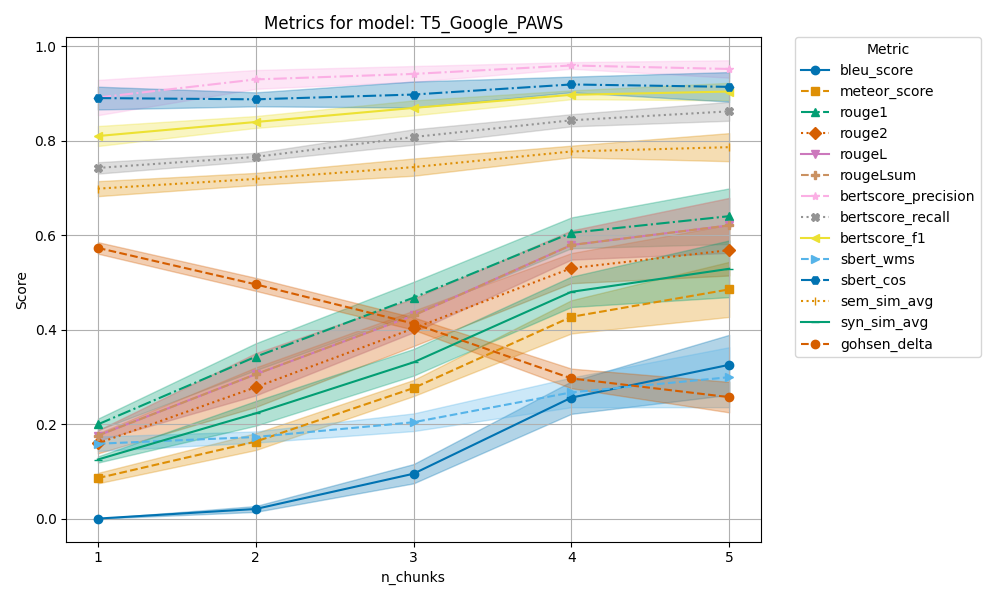
\includegraphics[width=\textwidth]{images/paraphrasing/experiments/T5_Google_PAWS_metrics_plot.png}
    \caption{Average score over different prompts (standard deviation shaded) for different paraphrasing scores for the \ac{t5} model.
    The syntactic scores rise with the number of chunks, while the semantic scores is stable.
    Consequently, the Gohsen Delta score is decreasing with the number of chunks.}
    \label{fig:abl_chunks_T5_Google_PAWS}
\end{figure}

\begin{figure}[htbp]
    \centering
    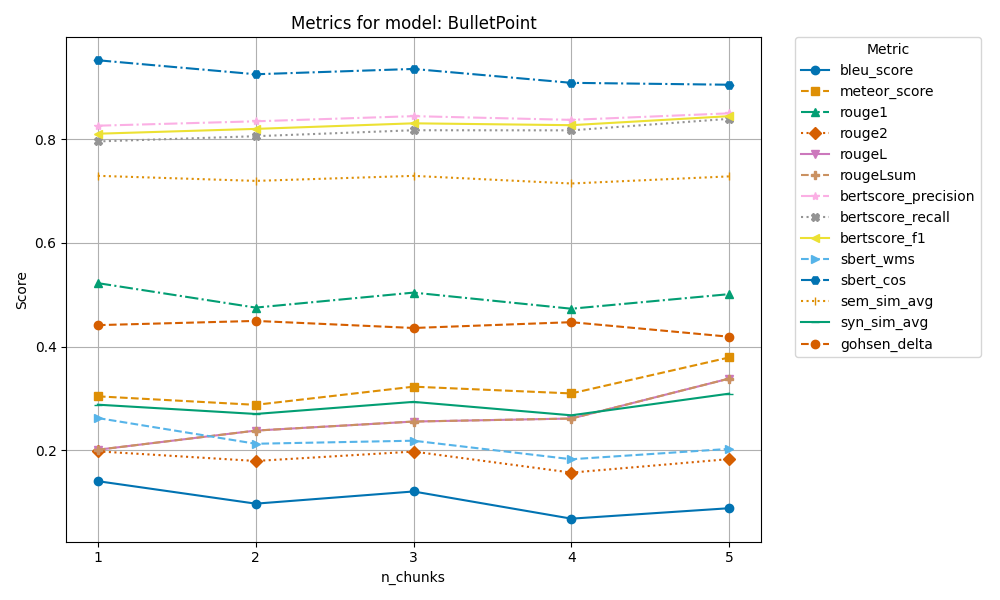
\includegraphics[width=\textwidth]{images/paraphrasing/experiments/BulletPoint_metrics_plot.png}
    \caption{Different paraphrasing scores for the BulletPoint model. 
    This model is not affected by the number of chunks.}
    \label{fig:abl_chunks_BulletPoint}
\end{figure}
    % \chapter{Conclusion \& Outlook}
\label{chap:conclusion_outlook}

    \chapter{Notes}
    % notes
    % using input to avoid pagebreaks

\section{\acs{pan}}
\label{sec:pan}

The \ac{pan} workshop series accommodates shared tasks % like kaggel competitions
on authorship analysis, computational ethics, and the originality of writing \cite{ayele_overview_2024}.
\ac{pan}'s goal is to contribute to reproducible research in the fields of \ac{ir} and \ac{nlp}.
Submissions are submitted to the submission software \tira{}.
Among others, the workshop includes the \textit{Generative \ac{ai} Authorship Verification} task, which focuses on the detection of \ac{ai}-generated text.

\section{\acs{pan} \ac{av}}
\label{sec:pan_authorship_verification}

\citet{ayele_overview_2024} provide \autoref{tab:hierarchy_authorship_verification_problems}, i.e., 
the decomposition of \ac{av} into multiple subtasks. 
They order the subtasks in terms of their complexity.
The first task on the one hand, is considered the easiest, since we know that out of two text, one is guaranteed to be human-generated while the other one is \ac{llm}-generated.
The last task on the other hand, is denoted as the most difficult, since we do not know whether the text is human- or \ac{llm}-generated.


\begin{table}[tbp]
    \centering
    \caption{Hierarchy of \ac{av} problems \citep{ayele_overview_2024,bevendorff_overview_2024} from easiest (1) to most difficult (7), 
    where A, B corresponds to human-authored text and M denotes \ac{llm}-generated text.}
    \label{tab:hierarchy_authorship_verification_problems}
    \resizebox{\textwidth}{!}{%
    \begin{tabular}{lll}
        \toprule
    \rowcolor[HTML]{EFEFEF} 
    \textbf{Difficulty} & \textbf{Input/ Task} & \textbf{Possible Assignment Patterns} \\  \midrule
    1 & \{?,?\} & \{A,M\} \\ 
    2 & \{?,?\} & \{A,M\}, \{A,A\} \\
    3 & \{?,?\} & \{A,M\}, \{M,M\} \\
    4 & \{?,?\} & \{A,M\}, \{A,A\}, \{M,M\} \\
    5 & \{?,?\} & \{A,M\}, \{A,A\}, \{A,B\} \\
    6 & \{?,?\} & \{A,M\}, \{A,A\}, \{A,B\}, \{M,M\} \\
    7 & ? & A, M \\ \bottomrule
    \end{tabular}%
    }       
\end{table}

\citet{boenninghoff_o2d2_2021} state that \ac{pan} moved from a cross-topic closed-set \ac{av} task 
to cross-topic open-set \ac{av} task over three years.

\citet{boenninghoff_o2d2_2021} formally define the task:
For two documents $D_1$ and $D_2$, ground-truth hypothesis $H_a$ for $a \in \{0,1\}$ 
where $a=1$ means that $D_1$ and $D_2$ are written by the same author and 
$a=0$ means that they are not written by the same author, find $f: \{D_1, D_2\} \rightarrow p \in [0,1]$.
The estimated label $\hat{a}$ is then determined by the threshold $\theta$ applied to $p$:
$$\hat{a}=\left\{ \begin{matrix}
1\text{ if }p > 0.5 \\
0\text{ if }p < 0.5 \\
non-response\text{ if }p\text{ close to }0.5
\end{matrix}\right\}$$
These rules lead to three hypotheses:
\begin{itemize}
    \item $H_0$: $D_1$ and $D_2$ are written by different authors
    \item $H_1$: $D_1$ and $D_2$ are written by the same author
    \item $H_2$: Undecidable, trial does not suffice to establish authorship
\end{itemize}
% acquisition
\citet{ayele_overview_nodate} collected articles of major 2021 US news from Google News.
They chose this time period since it predates the release of GPT-3.5.
As a consequence, they claim that their dataset is most likely human-authored.
% artificial texts
Next, they used GPT-4-Turbo to create bullet-point summaries of the articles. 
Based on these summaries, 15 \acp{llm}-generated newspaper articles.
% split
The authors split the dataset into training and test set.
% robustness
In order to test the submissions' robustness, \citet{ayele_overview_nodate} generated 65 variants of the newspapers in the test split.
These variants include:
\begin{enumerate}
    \item Change English to German texts
    \item Replace 15\% of the characters
    \item Shuffling test case pairs to break topic coherence \todo{macht es das nicht leichter?}
    \item Contrastive decoding instead of top-k/top-p sampling
    \item Cropping texts to 35 words
    \item Using the prompt from a previous Kaggle competition on \ac{llm} detection to generate more faithful paraphrases of the original articles
\end{enumerate}
\section{\acs{pan} evaluation}
\label{sec:pan_evaluation}

\citet{ayele_overview_nodate} evaluate the participants submissions averaging the datasets' evaluation measures.
They claim the following measures are established in authorship verification:
\begin{itemize}
    \item \ac{roc-auc}
    \item BRIER
    \item C@1
    \item $F_1$
    \item $F_{0.5u}$
\end{itemize}

    \section{Definitions}
\label{sec:definitions}


% \begin{definition}
%     []
% \end{definition}

\begin{definition}
    [Text]
    A sequence of tokens or characters grouped into sentences \cite{elmanarelbouanani_authorship_2014}.
\end{definition}

\begin{definition}
    [Token]
    A token can be a word, a number or a punctuation mark \cite{elmanarelbouanani_authorship_2014}.
\end{definition}

\begin{definition}
    [Monograph]
    Single author document \cite{bevendorff_smauc_2023}.
\end{definition}

\begin{definition}
    [Multi-author (i.e. Collaborative) publication]
    Document with multiple authors \cite{bevendorff_smauc_2023}.
\end{definition}

\begin{definition}
    [Author profiling]
    Task of inferring an extensive set of (sensitive) personal information.
    This includes sociolinguistic attributes like age, gender, occupation, education, socio-economic status, cultural background, 
    language familiarity and mental health issues 
    \cite{emmery_adversarial_2021,stamatatos_survey_2009,elmanarelbouanani_authorship_2014}.
    The task is also referred to as author characterization \cite{stamatatos_survey_2009,elmanarelbouanani_authorship_2014}.
\end{definition}

\begin{definition}
    [Stylometry]
    Liguistic research area, which refers to the (statistical) analysis of authorial/ literally style \cite{elmanarelbouanani_authorship_2014,neal_surveying_2018}.
    Stylometry assumes that style is quantifiably measurable for evaluation of distinctive qualities and 
    that features, such as subconscious syntactic idiosyncrasies are sufficient in defining an author's unique style \cite{neal_surveying_2018}.
    The construction of models for the quantification of writing style, text complexity, and grading level assessment.
    Stylometric features include lexical, syntactic and structural features \cite{stein_intrinsic_2011}.
    In other words, stylometry is the statistical analysis of literary style between one writer or genre and another \cite{tyo_state_2022}.
    Research includes five subtasks \cite{neal_surveying_2018}:
    \begin{itemize}
        \item \ac{aa}
        \item \ac{av}
        \item Author profiling
        \item Stylochronometry
        \item adversarial stylometry
    \end{itemize}
\end{definition}

\begin{definition}
    [Stylochronometry]
    The study and detection of changes in authorial style over time \cite{neal_surveying_2018}.
\end{definition}

\begin{definition}
    [Stylistics]
    The study of stylometric features \cite{elmanarelbouanani_authorship_2014,abbasi_writeprints_2008}.
\end{definition}

\begin{definition}
    [Author writing style]
    Among others, syntactic structure of sentences in a document \cite{jafariakinabad_self_supervised_2022}.
    Opposed to other text categorization tasks, features do not include content \cite{koppel_authorship_2004}.
\end{definition}

\citet{elmanarelbouanani_authorship_2014} claim there are four (five \cite{abbasi_writeprints_2008,neal_surveying_2018}) types of writing style/ stylistic features:
\begin{itemize}
    \item Lexical features \citet{elmanarelbouanani_authorship_2014,abbasi_writeprints_2008,neal_surveying_2018}
    \item Syntactic features \citet{elmanarelbouanani_authorship_2014,abbasi_writeprints_2008,neal_surveying_2018}
    \item Structural features \citet{elmanarelbouanani_authorship_2014,abbasi_writeprints_2008,neal_surveying_2018}
    \item Content/Domain-specific features \citet{elmanarelbouanani_authorship_2014,abbasi_writeprints_2008,neal_surveying_2018}
    \item Idiosyncratic features \citet{abbasi_writeprints_2008}
    \item Semantic features \cite{neal_surveying_2018}
\end{itemize}

\begin{definition}
    [Online stylometric analysis]
    The analysis of authors style in online texts \cite{abbasi_writeprints_2008}.
    \citet{abbasi_writeprints_2008} define online texts as any textual documents that may be found in an online setting, 
    including computer-mediated communication, non-literary electronic documents (e.g., student essays, mews, articles, etc.), and program code.
\end{definition}

\begin{definition}
    [Style markers]
    Taxonomies of features to quantify the writing style \cite{stamatatos_survey_2009}.
\end{definition}

\begin{definition}
    [Stylistic features]
    Features that are the attributes or writing-style markers that are the most effective discriminators of authorship \cite{abbasi_writeprints_2008}.
\end{definition}

\begin{definition}
    [Lexical features]
    Lexical features are common features used in stylometry.
    They are character- (i.e. character (n-gram) frequency, ...) 
    or word-based (i.e. average word~\cite{stein_intrinsic_2011}, sentence length~\cite{stein_intrinsic_2011,abbasi_writeprints_2008}, 
    line length~\cite{abbasi_writeprints_2008}, word length distribution~\cite{abbasi_writeprints_2008}, 
    vocabulary richness~\cite{abbasi_writeprints_2008,neal_surveying_2018} ...) features. 
    These features consider text as a mere sequence of word-tokens or characters, respectively \cite{stamatatos_survey_2009}.
    Word features are more complex than character features \cite{stamatatos_survey_2009}.
    Character features are language-independent, not highly affected by noise (compared to word features), 
    and do not require natural language processors \cite{neal_surveying_2018}.
\end{definition}

\begin{definition}
    [Syntactic features]
    Syntactic features include function words, punctuation, and \ac{pos} tag $n$-grams \cite{abbasi_writeprints_2008}.
    They are language-dependent and require natural language processors \cite{neal_surveying_2018}.
\end{definition}

\begin{definition}
    [Semantic features]
    Semantic features capture meaning behind words, phrases, and sentences, such as through analysis of synonyms and semantic dependencies \cite{neal_surveying_2018}.
\end{definition}

\begin{definition}
    [Structural features]
    Structural features include text organization, layout, file extensions, font, sizes, colours, 
    use of braces and comments (for analysing computer programs) \cite{abbasi_writeprints_2008,neal_surveying_2018}.
\end{definition}

\begin{definition}
    [Content-specific features]
    Content-specific features include important keywords and phrases on certain topics such as word $n$-grams \cite{abbasi_writeprints_2008}.
    Domain-specific features include ratios of quoted words and external links, number of paragraphs, 
    and paragraphs average length for the news article domain \cite{potthast_stylometric_2018}
\end{definition}

\begin{definition}
    [Idiosyncratic features]
    Idiosyncratic features include misspellings, grammatical mistakes, and other usage anomalies \cite{abbasi_writeprints_2008,neal_surveying_2018}.
    Such features are extracted using spelling and grammar checking tools and dictionaries \cite{abbasi_writeprints_2008}.
\end{definition}

\begin{definition}
    [Feature-set type]
    There are two types of feature sets \cite{abbasi_writeprints_2008,neal_surveying_2018}:
    \begin{itemize}
        \item Author-group-level where one set of features is applied across all authors.
        \item Individual-author-level where each author has a unique set of features (e.g., 10 authors = 10 feature sets; 5000 most frequent character $n$-grams per author).
    \end{itemize}
    Individual-author-level features are effective for feature categories with potentially large feature spaces, such as $n$-grams or misspellings \cite{abbasi_writeprints_2008}.
    However, standard machine learning techniques typically require a fixed feature set for all authors \cite{abbasi_writeprints_2008}.
    Traditional single-author-group-level feature sets include \acp{svm} and \ac{pca} \cite{abbasi_writeprints_2008}.
\end{definition}

\begin{definition}
    [Static features]
    Static features include context-free categories such as function words, 
    word-length distributions, vocabulary richness measures, etc. \cite{abbasi_writeprints_2008}.
\end{definition}

\begin{definition}
    [Dynamic features]
    Dynamic features are context-dependent attributes and include $n$-grams and misspelled words \cite{abbasi_writeprints_2008}.
\end{definition}

\begin{definition}
    [Stability]
    Stability refers to how often a feature changes across authors and documents for a constant topic.
    \citet{abbasi_writeprints_2008} state that nouns are more stable than function words and thus, 
    function words are better stylistic discriminators than nouns 
    since using function words involves making choices between sets of synonyms.
\end{definition}

\begin{definition}
    [Adversarial Stylometry]
    Attack models that automatically infer a variety of potentially sensitive author information \cite{emmery_adversarial_2021} 
    via alteration of one's style \cite{neal_surveying_2018}.
    These attacks are not to be confused with adversarial learning \cite{emmery_adversarial_2021}.
    There are three forms of adversarial stylometry \cite{neal_surveying_2018}:
    \begin{itemize}
        \item Imitation: Writing to closely match the style of another author.
        \item Translation: Machine translating the language of a document to another language and back to the original language one or multiple times.
        \item Obfuscation: Paraphrasing such that the meaning of the text is preserved, but the style is changed.
    \end{itemize}
\end{definition}

\begin{definition}
    [Closed world]
    In the realm of plagiarism detection, closed world refers to the assumption 
    that a reference collection $D$ of documents, 
    that are supposed to be compared to the possibly plagiarized text, is given \cite{stein_intrinsic_2011}.
    In the realm of \ac{av} and \ac{aa} texts in the test set are assumed to be written by one of the authors in the training set \cite{boenninghoff_o2d2_2021,neal_surveying_2018}.
\end{definition}

\begin{definition}
    [Plagiarism]
    In the context of texts, plagiarism is the usage of another author's information, language, 
    or writing without properly acknowledging the original source \cite{stein_intrinsic_2011}.
    \citet{elmanarelbouanani_authorship_2014} define plagiarism as the complete or partial replication 
    of a piece of work with or without permission of the original author.
\end{definition}

\begin{definition}
    [Plagiarism detection]
    The task of identifying plagiarized text \cite{stein_intrinsic_2011}, i.e. finding similarities between two texts \cite{stamatatos_survey_2009}.
    Plagiarism detection uses similarity detection, determining whether multiple pieces of work were produced by a single author 
    without necessarly identifying the author \cite{elmanarelbouanani_authorship_2014}.
\end{definition}

\begin{definition}
    [Intrinsic plagiarism detection]
    This task can be understood as a more general form of \ac{av}.
    By analysing undeclared changes in writing style, potential plagiarism can be detected.
    Opposed to \ac{av}, where the decision is made based on the whole text, 
    intrinsic plagiarism detects plagiarism on a section level \cite{stein_intrinsic_2011}.
    Intrinsic analysis does not use any information on authorship from external sources \cite{zangerle_overview_2024}.
\end{definition}

\begin{definition}
    [Authorship analysing]
    This problem devises into two \textcolor{orange}{(i.e. first two acc. to \cite{stein_intrinsic_2011}, all acc. to \cite{stamatatos_survey_2009})} subtasks \cite{stein_intrinsic_2011}:
    \begin{itemize}
        \item \ac{aa} \cite{stein_intrinsic_2011}
        \item \ac{av} \cite{stein_intrinsic_2011,stamatatos_survey_2009}
        \item Plagiarism detection \cite{stamatatos_survey_2009}
        \item Author profiling \cite{stamatatos_survey_2009}
        \item Detection of stylistic inconsistencies (i.e. in collaborative writing) \cite{stamatatos_survey_2009}
    \end{itemize}
\end{definition}

\begin{definition}
    [\ac{aa}]   % authorship attribution
    The task of determining the author of a text based on textual features 
    given a (canonical) set of candidate authors with undisputed writing samples 
    \cite{stein_intrinsic_2011,koppel_authorship_2004,stamatatos_survey_2009,tyo_state_2022,bischoff_importance_2020,barlas_cross_domain_2020,altakrori_topic_2021,bevendorff_divergence_based_2020,elmanarelbouanani_authorship_2014,abbasi_writeprints_2008,llm_detection_av_2025,neal_surveying_2018}.
    The decision is made based on stylistic traits rather than the content of the document \cite{neal_surveying_2018}.
    In terms of machine learning, this is a multiclass, single-label text categorization task 
    \cite{stamatatos_survey_2009,koppel_authorship_2004,elmanarelbouanani_authorship_2014} 
    or text classification task \cite{elmanarelbouanani_authorship_2014}.
    The task is also referred to as author(ship) identification \cite{stamatatos_survey_2009,elmanarelbouanani_authorship_2014}.
    \citet{barlas_cross_domain_2020} express the \ac{aa} task as a tuple $(A,K,U)$, 
    where $A$ is the set of authors, $K=\underset{a\in A}{\cup}K_a$ is the set of known texts and $U$ is the set of unknown texts.
    If closed-set \ac{aa}: Each text $d \in U$ is attributed to exactly one author $a \in A$.
    If cross-topic(/-genre) \ac{aa}: The topic(/genre) of documents in $d \in U$ is distinct 
    with respect to the topics(/genres) found in $K$ \cite{barlas_cross_domain_2020}. 
    \citet{llm_detection_av_2025,neal_surveying_2018} state that \ac{aa} with few (<20) candidate authors is typically highly effective, 
    even if only short writing samples are available \cite{llm_detection_av_2025}/ 
    where each author has training samples of at least 1000 words \cite{neal_surveying_2018}.
    Many candidate authors impede the \ac{aa} problem.
    Models that abstain in uncertain many candidates scenarios still achieve good results \cite{llm_detection_av_2025}.
    $k$-attribution/ ranking (i.e. relaxed \ac{aa}, where the classifier output the top $k$ authors ranked by their probability of being the author of the text), 
    cross-domain/ cross-genre \ac{aa} (i.e., identify author $M$ of document written in domain $A$, while only having documents from $m$ in domain $B$ and thus, 
    features of domain $B$ must be applicable to domain $A$), 
    and source code \ac{aa} 
    are forms of \ac{aa} \cite{neal_surveying_2018}.
\end{definition}

\citet{elmanarelbouanani_authorship_2014} describe the workflow of \ac{aa} as follows:
\begin{enumerate}
    \item Data cleaning
    \item Feature extraction
    \item Normalization
    \item Converting each text into a feature vector, where author is the class label
    \item Split the dataset into training and test set
\end{enumerate}
Common classifiers include \ac{svm}, decision trees, and \acp{nn} \cite{elmanarelbouanani_authorship_2014}.

\begin{definition}
    [\ac{av}]   % authorship verification
    Given a set of writing samples of author $A$ and a text $t$,    % tyo_state_2022: only one wrinting sample
    the task is to determine whether $t$ was written by $A$ \cite{stein_intrinsic_2011,stamatatos_survey_2009,koppel_authorship_2011,tyo_state_2022,kocher_unine_2015,koppel_authorship_2004}.
    This task can also be formulated as whether two texts $t_1$ and $t_2$ are written by the same author 
    \cite{bevendorff_generalizing_2019,bevendorff_divergence_based_2020,embarcadero_ruiz_graph_based_2022,rivera_soto_learning_2021,ordonez_will_2020,futrzynski_pairwise_2021,weerasinghe_feature_vector_difference_2021,llm_detection_av_2025}.
    % Gespräch Martin Potthast 19.05.2025: problem formulation 2 is less common and in the context of very sparse (metadata) information
    Related research areas include \cite{stein_intrinsic_2011}:
    \begin{itemize}
        \item stylometry
        \item outlier analysis and meta learning
        \item symbolic knowledge representation, i.e. \todo{knownledge representation, deduction, heuristic inference}
    \end{itemize}
    \citet{tyo_state_2022} state that \ac{av} is the fundamental problem of \ac{aa} \cite{tyo_state_2022}, 
    where there is only one candidate author \cite{barlas_cross_domain_2020}.
    \citet{llm_detection_av_2025,koppel_authorship_2004} state that \ac{av} is a more general and difficult (than \ac{aa}) one-class classification problem.
    Hence, the disputed document is compared only to documents from the candidate, 
    ignoring intermediate negatives (all human texts not written by the known author) 
    \cite{llm_detection_av_2025,neal_surveying_2018,koppel_authorship_2004}.
    It is impossible to assemble an exhaustive, or even representative samples of the non-target class \cite{koppel_authorship_2004}.
    \ac{av} is different from usual one-class classification problems, in which there is a lack of negative examples (opposed to non-representative ones), 
    and in which the text to attribute is not necessarily long (opposed to \citet{koppel_authorship_2004}'s paper).
    \citet{neal_surveying_2018} consider \ac{av} a binary classification problem (i.e. \textit{same-author} or \textit{different-author}), 
    where \textit{different-author} renders \ac{av} as an open-set problem.
    However, \citet{neal_surveying_2018} consider framing \ac{av} as a one-class classification problem as a common approach (cf. \cite{llm_detection_av_2025}).
    \citet{elmanarelbouanani_authorship_2014} consider \ac{av} a similarity detection task.
    \citet{neal_surveying_2018} also mention the many-candidates method where \ac{av} is framed as \ac{aa} via creating a set of imposters.
    Use cases include plagiarism detection, moderation of user-generated content, historical \ac{aa}, and forensic analysis \cite{rivera_soto_learning_2021}.
\end{definition}

\begin{definition}
    [Similarity detection]
    The task of comparing anonymous texts against other anonymous texts to assess the degree of similarity in terms of stylistic characteristics \cite{abbasi_writeprints_2008,neal_surveying_2018}.
    In the context of \ac{av}, the task is to determine whether two texts are produced by the same person without knowing the real author of the document \cite{elmanarelbouanani_authorship_2014}.
\end{definition}

\begin{definition}
    [Message-level analysis]
    The analysis attempts to categorize individual texts (e.g., whether an email was authored by an email address) \cite{abbasi_writeprints_2008}.
\end{definition}

\begin{definition}
    [Identity-level analysis]
    The analysis attempts to classify individuals belonging to a particular entity 
    (e.g., whether different email addresses belong to the same entity).
    Identity-level analysis' categorization is based on all texts written by that identity.
    Hence, there are larger text samples than for message-level analysis, facilitating the task.
    If the task is framed as classification/ID identification, the disputed identity is assigned to the identity with the highest similarity among the known identities.
    If the task is framed as similarity detection task, all identities with a similarity score above a certain threshold are grouped together and 
    considered to belong to the same entity \cite{abbasi_writeprints_2008}.
\end{definition}

\begin{table}[]
    \centering
    \caption{Building blocks for \ac{av} from \cite{stein_intrinsic_2011}.}
    \label{tab:authorship_verification_blocks}
    \resizebox{\textwidth}{!}{%
    \begin{tabular}{|l|lll|l|}
    \hline
    \rowcolor[HTML]{EFEFEF} 
    Pre-analysis & \multicolumn{3}{l|}{\cellcolor[HTML]{EFEFEF}Modeling and classifier methods} & Post-processing \\ \hline
    \rowcolor[HTML]{EFEFEF} 
    Impurity assessment & \multicolumn{1}{l|}{\cellcolor[HTML]{EFEFEF}Decomposition strategy} & \multicolumn{1}{l|}{\cellcolor[HTML]{EFEFEF}Style model construction} & Outlier identification & Outlier post-processing \\ \hline
    Document length analysis & \multicolumn{1}{l|}{Uniform length} & \multicolumn{1}{l|}{Lexical character features} & One-class density estimation & Heuristric voting \\
    Genre Analysis & \multicolumn{1}{l|}{Structural boundaries} & \multicolumn{1}{l|}{Lexical word features} & One-class boundary estimation & Citation analysis \\
    Analysis of issuing institution & \multicolumn{1}{l|}{Text element boundaries} & \multicolumn{1}{l|}{Syntactical features} & One-class reconstruction & Human inspection \\
     & \multicolumn{1}{l|}{Topical boundaries} & \multicolumn{1}{l|}{Structural features} & Two-class discrimination & Unmasking \\
     & \multicolumn{1}{l|}{Stylistic boundaries} & \multicolumn{1}{l|}{Language modeling} &  & Qsum \\
     & \multicolumn{1}{l|}{} & \multicolumn{1}{l|}{} &  & Batch means
    \end{tabular}%
    }
\end{table}
Post-processing to avoid false positives, c.f. \citet{stein_intrinsic_2011} for approaches.

\begin{definition}
    [Meta learning]
    \todo{Based on learning successes and failures, the system learns to learn. }
    Approaches include:
    \begin{itemize}
        \item Unmasking: Measurement of reconstruction errors starting from a good reconstruction and iteratively impairing the reconstruction. % example on page 9 of Benno's paper
        \item Qsum heuristic: Compares the growth rates of two cumulative sums over a sequence of sentences. The sums are calculated via the deviations from the mean sentence length and the deviations of the function words.
        \item Batch means: \todo{For a series of values the variance development of the sample mean is measured while the sample size is successively increased.}
    \end{itemize}
\end{definition}

\begin{definition}
    [Unmasking]
    The idea of this meta learning approach is that with progressively omitting more and more frequent words/ 
    most discriminating features, 
    topic specific words are excluded and thus, leaving only writing style specific words \cite{stein_intrinsic_2011}.
    After several iterations, remaining features which are not powerful enough to discriminate two documents indicate that 
    these documents originate from the same author \cite{stein_intrinsic_2011,tyo_state_2022,bevendorff_divergence_based_2020,koppel_authorship_2004}.
    In other words: 
    Two texts are probably written by different authors if the differences between are robust to changes in the underlying feature set used to represent the documents.
    Differences can be measured using instance-based (meta) classification via cross-validation accuracy 
    \cite{koppel_authorship_2011,bevendorff_generalizing_2019,bevendorff_divergence_based_2020,potthast_stylometric_2018,koppel_authorship_2004}, 
    creating a performance degradation curve \cite{tyo_state_2022,koppel_authorship_2004}.
    An \ac{svm} is trained to classify the degradation curve to determine whether two text originated from the same author 
    \cite{tyo_state_2022,bevendorff_generalizing_2019,koppel_authorship_2004}.
    Cf. \cite{bevendorff_divergence_based_2020} Chapt. 2 for a detailed algorithm.
    Steep decrease in the curve indicates that the two texts are similar, and thus, 
    written by the same authors \cite{potthast_stylometric_2018,koppel_authorship_2004}.
    Provided that the unseen text is very large, this method can handle small open candidate sets \cite{koppel_authorship_2011}.
    % koppel_determining_2014, pg. 1 + bevendorff_generalizing_2019 chap. 3.1 incl. algo: based on text chunks of length >= 500 words each
    \citet{koppel_determining_2014,bevendorff_generalizing_2019} claim that effective unmasking requires input documents to be large 
    (i.e. > 10000 words~\cite{koppel_determining_2014}, book-length~\cite{bevendorff_generalizing_2019}, 
    $\geq$ 5000 words (500 words per chunk) \cite{bevendorff_divergence_based_2020}).
    Otherwise the training set becomes too sparse and no descriptive curves can be generated 
    \cite{bevendorff_generalizing_2019,bevendorff_divergence_based_2020}.
\end{definition}

\begin{definition}
    [Stop words vs. function words]
    Function words are the most common words (articles, prepositions, pronouns, etc.) 
    like "while", "upon", "though", "were", "your" \cite{stamatatos_survey_2009,elmanarelbouanani_authorship_2014}.
    They are typically regarded as context-free (and therefore less influenced by topic and genre), 
    while revealing social and personal aspects of our lives \cite{neal_surveying_2018}.
    Most function words are stop words, but not all stop words are function words \cite{stein_intrinsic_2011}.
    \citet{elmanarelbouanani_authorship_2014} state that researchers use between 150 and 675 function words as features.
    \citet{abbasi_writeprints_2008} state that function words are highly effective discriminators of authorship, since 
    the usage variations of such words are strong reflection of stylistic choices.
\end{definition}

\begin{definition}
    [One-class classification]
    A classification problem where the classifier is trained on samples of a single class.
    If counterexamples, i.e. so-called outliers, are available, they are usually not considered to be representative of \textit{non-target class}.
    Hence, the classifier has to learn the concept of the target class in the absence of discriminating features 
    \cite{stein_intrinsic_2011,koppel_authorship_2004}.
    Examples of one-class classification are intrinsic plagiarism analysis and \ac{av}.
    Approaches to one-class classification fall into the following categories \cite{stein_intrinsic_2011}:
    \begin{itemize}
        \item One-class density estimation, e.g., Naive Bayes
        \item One-class boundary estimation
        \item One-class reconstruction
    \end{itemize}
\end{definition}

\begin{definition}
    [Open-set classification]
    The true author is not necessarily included in the set of candidate authors \cite{stamatatos_survey_2009,barlas_cross_domain_2020,neal_surveying_2018}.
    It is a generalization of the closed-set classification problem allowing for an unknown author using a threshold for similarity \cite{neal_surveying_2018}.
\end{definition}

\begin{definition}
    [Closed-set classification]
    The true author is one necessarily one of the candidate authors \cite{stamatatos_survey_2009,koppel_authorship_2011,barlas_cross_domain_2020,boenninghoff_o2d2_2021,neal_surveying_2018}.
    In other words: The set of all possible author classes is known a priori.
    Hence, closed-set problems can use supervised or unsupervised classification techniques \cite{abbasi_writeprints_2008}.
\end{definition}

\begin{definition}
    [Supervised techniques]
    Supervised techniques for stylometric analysis require (author-)class labels for categorization.
    Examples include \acp{svm}, \acp{nn}, decision trees, and linear discriminant analysis.
    \acp{svm} are very common in authorship analysis due to their robustness \cite{abbasi_writeprints_2008}.
\end{definition}

\begin{definition}
    [Unsupervised techniques]
    Unsupervised techniques make categorizations with no prior knowledge of author classes.
    Examples include \ac{pca} and cluster analysis.
    \ac{pca} has been used in previous authorship studies due to its ability to 
    capture essential variance across large number of features in a reduced dimensionality \cite{abbasi_writeprints_2008}.
\end{definition}

\begin{definition}
    [Covariate shift]
    The distribution of neural stylometric features changes between training and test set due to, for instance, topic variability \cite{boenninghoff_o2d2_2021}.
\end{definition}

\begin{definition}
    [n-gram]
    $n$ contiguous words also known as word collocations. \todo{cite, reference?\cite{koppel_authorship_2011}?}
    n-grams are no stylometric features \cite{altakrori_topic_2021}.
    % Quelle Martin Potthast Gespräch 19.05.2025:
    Tri-grams are commonly used in stylistic analysis, due to their ability to capture inflections, % Flexion/ Beugung in Deutsch
    morphemes, %  smallest meaningful constituents within a linguistic expression and particularly within a word
    and other syntactic structures for Germanic languages.
    Character-level $n$-gram features capture the frequency of $n$ consecutive characters in a text \cite{neal_surveying_2018}.
    The optimal $n$ is language dependent \cite{neal_surveying_2018}.
\end{definition}

\begin{definition}
    [Space free n-gram]
    Removing spaces from the $n$-gram reduces the number of $n$-grams.
    \citet{koppel_authorship_2011} use these definitions:
    \begin{enumerate}
        \item a string of $n$ characters that not include spaces
        \item a string of less than $n$ characters that is surrounded by spaces
    \end{enumerate}
\end{definition}

\begin{definition}
    [Domain shift]
    Systematic statistical differences between the training and test sets \cite{tyo_state_2022}.
    These differences include:
    \begin{itemize}
        \item datasets are not identically distributed
        \item test set contains novel topics $\times_t$
        \item test set contains novel authors $\times_a$
        \item test set contains novel genres $\times_g$
    \end{itemize}
\end{definition}

\begin{definition}
    [Topic-confusion]
    In this setting, all topics appear in both training and test set. 
    However, the topics of the texts for each author changes in the test set, 
    i.e. author-topic configuration is switched between training and testing.
    For example, in the training set, the author $A_1$ writes about topic $T_1$, author $A_2$ writes about topic $T_2$ 
    and in the test set, 
    the author $A_1$ writes about topic $T_2$ while author $A_2$ writes about topic $T_1$ \cite{tyo_state_2022,altakrori_topic_2021}.
    Intuitive, the more a feature is influenced by the topic of document to identify its author, 
    the more confusion it will be to the classifier when the topic-author combination is switched, which will lead to performance deterioration \cite{altakrori_topic_2021}.
\end{definition}

\begin{definition}
    [text distortion]
    This domain-adversial method substitutes out-of-vocaublary items with asterisks $*$ \cite{tyo_state_2022}.
    Its goal is to reduce domain-specific information \cite{bischoff_importance_2020}.
    Distortion algorithms include \cite{bischoff_importance_2020}:
    \begin{itemize}
        \item Replacing tokens with multiple asterisks
        \item Replacing tokens with single asterisks
        \item Retaining only exterior characters of words in a dictionary
        \item Retaining the last two characters
    \end{itemize}
\end{definition}

\begin{definition}
    [Imposter method]
    This method extends the ngram-unmasking method, i.e. iteratively omitting most influencely features (repeated feature subsampling \cite{koppel_determining_2014})
    from a trained classifier and classifying the accuracy drop.
    It takes score of how often an author is predicted after each feature-elimination step.
    The final prediction is made based on this score \cite{tyo_state_2022}.
\end{definition}


\begin{definition}
    [Hard Negative Mining]
    This method updates the model during training only with the most difficult examples in each batch.
    In the \ac{aa} context, difficult is defined as the most similar two texts from different authors, 
    which makes the decision the most difficult.
    \citet{tyo_state_2022} claim that the \ac{av} setting is strictly easier since 
    it most compare to only a single text.
    Due to the fact, that the most difficult example is model-dependent, \ac{av} problems can be made harder 
    but they can not exist of exactly the hardest negatives.
\end{definition}

\begin{definition}
    [Domain]
    The domain include topic, genre, register, idiolect, time period etc. \cite{bischoff_importance_2020}.
\end{definition}
  
\begin{definition}
    [Domain variables]
    These include topic, genre and language \cite{bischoff_importance_2020}.
\end{definition}

\begin{definition}
    [Style transfer]
    Translation or rather paraphrasing a text from a source style to a desired target style.
    Two major problems include the lack of large-scale parallel training data (i.e., texts written in both styles), 
    and the lack of reliable evaluation metric (i.e. assessment by humans) \cite{bischoff_importance_2020}.
\end{definition}

\begin{definition}
    [Author obfuscation]
    Task of paraphrasing a text to render an author's style imperceptible.
    Usually, another text from the author is used as a reference for style similarity \cite{bischoff_importance_2020}.
    In other words: It is the adversarial task of preventing successful verification by altering the text's style so that 
    it no longer resembles the original author's style \cite{bevendorff_divergence_based_2020}.
\end{definition}

\begin{definition}
    [within-domain]
    Experiments with P=Q.
    Hence, it is necessary to ensure all texts are mutually from the same domain \cite{bischoff_importance_2020}.
    \begin{table}[]
        \centering
        \caption{Typical scheme $S_1$ for \ac{aa} problem instances, where A, B, are authors and P, Q domains and 
        the vertical mapping denotes which author has written in which domain. 
        For training, texts from A and B take turn; for testing, previously unseen texts from A and B are used \cite{bischoff_importance_2020}.}
        \label{tab:within_domain_aa}
        \begin{tabular}{|l|ll|ll|}
        \hline
        \textbf{Scheme $S_1$} & \multicolumn{2}{l|}{\textbf{training}} & \multicolumn{2}{l|}{\textbf{testing}} \\ \hline
        \textbf{authors} & \multicolumn{1}{l|}{A} & B & \multicolumn{1}{l|}{A} & B \\ \hline
        \textbf{domains} & \multicolumn{1}{l|}{P} & Q & \multicolumn{1}{l|}{P} & Q \\ \hline
        \end{tabular}%
    \end{table}
\end{definition}

\begin{definition}
    [Domain swapping]
    Experiments with P$\neq$Q \cite{bischoff_importance_2020}.
    \begin{table}[]
        \centering
        \caption{Domain-swapping scheme $S_2$ for \ac{aa} problem instances, where A, B, are authors and P, Q domains and 
        the vertical mapping denotes which author has written in which domain. 
        For training, texts from A and B take turn; for testing, previously unseen texts from A and B are used \cite{bischoff_importance_2020}.}
        \label{tab:within_domain_aa}
        \begin{tabular}{|l|ll|ll|}
        \hline
        \textbf{Scheme $S_2$} & \multicolumn{2}{l|}{\textbf{training}} & \multicolumn{2}{l|}{\textbf{testing}} \\ \hline
        \textbf{authors} & \multicolumn{1}{l|}{A} & B & \multicolumn{1}{l|}{A} & B \\ \hline
        \textbf{domains} & \multicolumn{1}{l|}{P} & Q & \multicolumn{1}{l|}{Q} & P \\ \hline
        \end{tabular}%
    \end{table}
    There are two kinds of domain swapping:
    \begin{itemize}
        \item \textbf{Zero-knowledge swapping}: Maximizes the potential for confusion during training, 
        since the models never see an author in writing in the other author's respective fandom.
        This approach aggravates adversarial training, since it needs domain knowledge to be effective.
        \item \textbf{High-imbalance swapping}: Imbalance is swapped between the training and test set. 
        This is an approximation of the zero-knowledge swapping, while still allowing adversarial learning.
    \end{itemize}
\end{definition}

\begin{definition}
    [train-test-validation split]
    \citet{bischoff_importance_2020,altakrori_topic_2021,boenninghoff_o2d2_2021} train their model on a selection of the dataset (i.e. training set), 
    optimize the model's hyperparameters on a second disjoint selection of the dataset (i.e. validation set),
    and evaluate the model on a third disjoint selection of the dataset (i.e. test set).
    \citet{bischoff_importance_2020} ensure that there is no data leakage between the training, validation and test sets 
    (i.e. prevent parts of one fanfiction being in more than one of the data splits).
    \citet{altakrori_topic_2021} ensure the classifier to be trained has no access to any information about the setup 
    (topic confusion: group configuration or topic labels).
\end{definition}

\begin{definition}
    [Cross-domain]
    Texts of known authorship (training set) differ from texts of disputed authorship (test set) 
    in topic (i.e. cross-topic) or genre (i.e. cross-genre) 
    \cite{barlas_cross_domain_2020}.
\end{definition}

\begin{definition}
    [Cross-topic]
    New, unseen topics are used in the testing phase \cite{altakrori_topic_2021}.
\end{definition}

% Please add the following required packages to your document preamble:
% \usepackage{graphicx}
\begin{table}[]
    \centering
    \caption{\ac{aa} scenarios with author $i$ is shortened with $A_i$ \cite{altakrori_topic_2021}.}
    \label{tab:aa_same_topic}
    \begin{tabular}{|l|l|l|}
    \hline
    \textbf{} & \textbf{Train} & \textbf{Test} \\ \hline
    \textbf{Topic $T_1$} & $A_1, A_2$ & $A_1, A_2$ \\ \hline
    \textbf{Topic $T_2$} & $A_1, A_2$ & $A_1, A_2$ \\ \hline
    \end{tabular}%
\end{table}

% Please add the following required packages to your document preamble:
% \usepackage{graphicx}
\begin{table}[]
    \centering
    \caption{\ac{aa} scenarios with author $i$ is shortened with $A_i$ \cite{altakrori_topic_2021}.}
    \label{tab:aa_cross_topic}
    \begin{tabular}{|l|l|l|}
    \hline
    \textbf{} & \textbf{Train} & \textbf{Test} \\ \hline
    \textbf{Topic $T_1$} & $A_1, A_2$ &  \\ \hline
    \textbf{Topic $T_2$} &  & $A_1, A_2$ \\ \hline
    \end{tabular}%
\end{table}

% Please add the following required packages to your document preamble:
% \usepackage{graphicx}
\begin{table}[]
    \centering
    \caption{\ac{aa} scenarios with author $i$ is shortened with $A_i$ \cite{altakrori_topic_2021}.}
    \label{tab:aa_topic_confusion}
    \begin{tabular}{|l|l|l|}
    \hline
    \textbf{} & \textbf{Train} & \textbf{Test} \\ \hline
    \textbf{Topic $T_1$} & $A_1$ & $A_2$ \\ \hline
    \textbf{Topic $T_2$} & $A_2$ & $A_1$ \\ \hline
    \end{tabular}%
\end{table}

\begin{definition}
    [Data preprocessing]
    Typical stylometry subtask for normalization and noise reduction.
    Examples include tokenization, stemming, tagging, removing non-alphabetic characters and spaces, and converting uppercase letters to lowercase \cite{neal_surveying_2018}.,
\end{definition}

\begin{definition}
    [Tokenization]
    Splitting a stream of text into words, phrases, etc. \cite{neal_surveying_2018}.
\end{definition}

\begin{definition}
    [Stemming]
    Only retaining the root or base form of a word \cite{neal_surveying_2018}.
\end{definition}

\begin{definition}
    [Tagging]
    Replacing words with their grammatical type \cite{neal_surveying_2018}.
\end{definition}

\begin{definition}
    [\ac{bow}]
    The \ac{bow} approach generally refers to lexical-level features as it represents a document as a bag (or collection) of words, 
    discarding context, grammar, and word order \cite{neal_surveying_2018}.
\end{definition}

\begin{definition}
    [Latent Dirichlet Allocation (LDA)]
    LDA is a three-level Bayesian technique for modelling a collection over a set of topics.
    LDA is a probabilistic model where each topic is determined by word distributions \cite{neal_surveying_2018}.
\end{definition}

\begin{definition}
    [Clustering]
    Clustering is an unsupervised machine-learning procedure, where the algorithm derives a natural separation of the feature space 
    that may or may not correlate with the class labels \cite{neal_surveying_2018}.
\end{definition}

\begin{definition}
    [Paraphrase divergence]
    This means that when a question is phrased in s slightly different but semantically similar way, 
    \ac{llm} may output a wrong response despite being able to answer to the original question correctly \cite{fu_learning_2024}.
\end{definition}

\begin{definition}
    [Paraphrases]
    Texts that convey identical meanings while using different words or (sentence) structures \cite{fu_learning_2024,zhou_paraphrase_2021,palivela_optimization_2021}.
\end{definition}

\begin{definition}
    [Encoder]
    The main purpose of an encoder is to extract the semantic information for the decoder \cite{zhou_paraphrase_2021}.
\end{definition}

\begin{definition}
    [Attention mechanism]
    Attention allows the model to focus on particular words/phrases in the input sequence when generating the output sequence.
    First, a weight (i.e. importance) for each token in the source sequence in each timestep is computed.
    Then, both the text input and the context vector with weights is provided to the decoder \cite{zhou_paraphrase_2021}.
\end{definition}

\begin{definition}
    [\acl{rl}]
    \ac{rl} trains agents to take actions in an environment to maximize a cumulative reward \cite{zhou_paraphrase_2021}.
\end{definition}

\begin{definition}
    [GANs]
    Generative Adversarial Networks (GANs) consist of a generator and a discriminator.
    The generator creates realistic data instances that match the real distribution, 
    while the discriminator distinguishes which instance are generated and which are real \cite{zhou_paraphrase_2021}.
\end{definition}

\begin{definition}
    [Zero-Shot]
    Zero-Shot capabilities enable models, e.g. \acp{llm}, to perform well on unseen tasks \cite{master_thesis_paraphrasing_2024}.
\end{definition}

\begin{definition}
    [Internal validity]
    Internal validity is the extent to which the study results can be attributed 
    to the manipulations of the independent variable rather than other factors \cite{master_thesis_paraphrasing_2024}.
\end{definition}

\begin{definition}
    [External validity]
    External validity is the extent to which the study results can be generalized 
    to other contexts, settings, or populations \cite{master_thesis_paraphrasing_2024}.
\end{definition}

\begin{definition}
    [Subtasks of Paraphrasing]
    There are two sub-tasks of paraphrasing \cite{palivela_optimization_2021}:
    \begin{itemize}
        \item \ac{pg}: The task of generating fluent and semantically similar paraphrases for a given sentence. 
        It can be solved by using simple lexical features and word ordering or restructuring methods or 
        by using templates extracted from WikiAnswers repositories \cite{palivela_optimization_2021}.
        Formally, for a sentence $S_1=\{w_1, \cdot, w_n\}$, generate one or more candidate sentences $S_2=\{w_1, \cdot, w_m\}, \cdot$.
        Sentence lengths may vary. \cite{palivela_optimization_2021}.
        \item \ac{pi}: The task of determining whether two sentences are paraphrases of each other.
        \ac{pi} ca be viewed as a discriminative task. The system output can be a probability (1 for paraphrase, 0 for non-paraphrase) 
        or a semantic score which can be normalized \cite{palivela_optimization_2021}.
        Formally, for a sentence pair $(S_1, S_2)$, find a target 1 or 0. Sentence lengths may vary. \cite{palivela_optimization_2021}.
    \end{itemize}
\end{definition}

\begin{definition}
    [Transfer learning]
    Transfer learning is a machine learning technique where a model trained on a data-rich task is 
    reused as the starting point (i.e. finetuning) for a model on a second task (i.e. downstream task) \cite{palivela_optimization_2021}.
\end{definition}

    Opposed to traditional vector space models, language models consider the context of a word when computing its embedding \cite{emmery_adversarial_2021}.


% BERT
\ac{bert} is a language model trained through masked language modelling and next-sentence prediction \cite{emmery_adversarial_2021}.
Hence, \citet{emmery_adversarial_2021}'s approach to substituting certain words in a text is straightforward:
The word to be substituted is masked, and the model predict the top-$k$ most likely words.
According to this approach two potential shortcomings arise:
\begin{itemize}
    \item The predicted word can be semantically inconsistent to the original.
    \item A semantic shift could occur since the model considers predicted words prior to the current word at each position.
\end{itemize}
\citet{emmery_adversarial_2021} propose mitigating these shortcomings by using dropout to zero part of the weights of the internal embedding of the target/ original word.
They assume that the top-$k$ candidate words are semantically more similar to the original word than the masked suggestions.
    An excessive amount of electronic texts is available on the internet.
Text categories include e-mail messages, online forum messages, blog posts and source code.
% obstacles
However, this data is prone to be noisy, short and from multiple candidate authors \cite{stamatatos_survey_2009}.
\section{Stylometric features}
\label{sec:stylometric_features}

Refer to \autoref{sec:definitions} for the definitions of the terms used in this section.

\begin{table}[]
    \centering
    \caption{Types of stylometric features with their computation tools and 
    resources where brackets indicate optional tools from \citep{stamatatos_survey_2009}.}
    \label{tabstylometric_features_tools}
    \resizebox{\textwidth}{!}{%
    \begin{tabular}{|l|l|l|}
    \hline
    \rowcolor[HTML]{EFEFEF} 
    \textbf{Category} & \textbf{Features} & \textbf{Required tools and resources} \\ \hline
    Lexical & Token-based (word/ sentence length, ...) & Tokenizer, (Sentence splitter) \\
     & Vocabulary richness & Tokenizer \\
     & Word frequencies & Tokenizer, (Stemmer, Lemmatizer) \\
     & Word n-grams & Tokenizer \\
     & Errors & Tokenizer, Orthographic spell checker \\
    Character & Character types (letters, digits, ...) & Character dictionary \\
     & Character n-grams (fixed length) & - \\
     & Character n-grams (variable length) & Feature selector \\
     & Compression methods & Text compression tool \\
    Syntactic & Part-of-Speech (POS) & Tokenizer, Sentence splitter, POS tagger \\
     & Chunks & Tokenizer, Sentence splitter, (POS tagger), Text chunker \\
     & Sentence and phrase structure & Tokenizer, Sentence splitter, POS tagger, Text chunker, Partial parser \\
     & Rewrite rule frequencies & Tokenizer, Sentence splitter, POS tagger, Text chunker, Full parser \\
     & Errors & Tokenizer, Sentence splitter, Syntactic spell checker \\
    Semantic & Synonyms & Tokenizer, (POS tagger), Thesaurus \\
     & Semantic dependencies & Tokenizer, Sentence splitter, POS tagger, Text chunker, Partial parser, Semantic Parser \\
     & Functional & Tokenizer, Sentence splitter, POS tagger, Specialized dictionaries \\
    Application-specific & Structural & HTML parser, Specialized parsers \\
     & Content-specific & Tokenizer, (Stemmer, Lemmatizer), Specialized dictionaries \\
     & Language-specific & Tokenizer, (Stemmer, Lemmatizer), Specialized dictionaries
    \end{tabular}%
    }
\end{table}
\citet{bevendorff_overview_2024} list lexical diversity, average sentence length, average word length, 
the number of grammatical errors, sentiment tendency, repetition rate, and stop word ratio as 
stylometric and linguistic features.

% all information from stamatatos_survey_2009
% lexical features
Lexical features consider sentences grouped sequences of tokens, i.e. words, numbers or punctuation marks \citep{bevendorff_overview_2024}.
They are used to learn about preferred use of characters and words of an author \citep{elmanarelbouanani_authorship_2014}.
% more lexical feature examples at elmanarelbouanani_authorship_2014 Ch. 3.1
% length counts
Simple attempts of author attribution include sentence lengths counts, and word length counts.
These approaches work straightforward assuming that the tokenizer is able to identify the tokens correctly \citep{bevendorff_overview_2024,elmanarelbouanani_authorship_2014}.
However, for some language such as Chinese, the tokenization is not trivial.
% vocabulary richness
Vocabulary richness functions attempt to quantify the diversity of vocabulary used in a text.
Approaches include $\frac{\text{size of vocabulary}}{\text{total number of tokens}}$ \citep{elmanarelbouanani_authorship_2014,bevendorff_overview_2024},
Yule's K measure \citep{elmanarelbouanani_authorship_2014},
the number of hapax legomena (words that occur only once in a text) \citep{elmanarelbouanani_authorship_2014,bevendorff_overview_2024,weerasinghe_feature_vector_difference_2021}, 
or the number of hapax dislegomena (words that occur twice in a text) \citep{elmanarelbouanani_authorship_2014,weerasinghe_feature_vector_difference_2021}.
The vocabulary size depends on the text length (quick increase in the beginning, slowly increasing later).
To mitigate this effect, researchers have proposed methods to introduce stability into these metrics \citep{elmanarelbouanani_authorship_2014,bevendorff_overview_2024}. 
According to \citet{stamatatos_survey_2009}, these proposed methods are questionable and should not be used alone.
\citet{neal_surveying_2018} list some of the most common vocabulary richness measures:
\begin{itemize}
    \item Zipf's law models a linear relationship between the number of vocabulary items appearing $r$ times in a document.
    \item Yule's K measure assumes that the occurrence of a word is based on chance and can be modelled according to a Poisson distribution.
    \item Yule's I measure $= \frac{M_1 M_1}{M_1 M_2}$, where $M_1$ is the number of words in a document and $M_2$ is the sum of weighted word forms with a certain frequency. A larger result indicates a richer vocabulary.
    \item The Burrows method considers large sets of high-frequency function words per 1000 words and then applies \ac{pca}. This method is considered a standard method in authorship attribution.
    \item Hapax legomena counts the number of words to appear one, while happax dislegomena counts the number of words to appear two times in a document.
    \item Type/token ratio is the ratio of all tokens (or words) to unique tokens (referred to as types).
\end{itemize}
% frequent words
\citet{elmanarelbouanani_authorship_2014} state that the most frequent words in a text is a lexical feature set.
% BoW
Texts can also be represented by vectors of word frequencies, i.e. the \ac{bow} model \citep{bevendorff_overview_2024}.
This representation disregards contextual, i.e., word-order, information.
While topic-based classification usually excludes so-called function words, 
i.e. most common words, since they do not carry any semantic information and are topic-independent, 
style-based text classification includes them.
In particular, function words are considered among the best features to discriminate between authors 
since they capture pure stylistic choices of authors across different topics.
Hence, style-based text classification requires much lower dimensionality (i.e., a few hundred words) 
in comparison to topic-based text classification (i.e., several thousand words).
Function words can be closed class words, i.e., articles, prepositions etc., 
or open-class words, i.e., nouns, adjectives, verbs.
Closed class words are the first dozen frequent words and 
open class words are predominantly present in the next frequent words.
% n-grams
To overcome the lack of contextual information in the \ac{bow} model, 
n-grams can be used.
However, the classification accuracy does not always increase with the usage of n-grams instead of individual word features.
Moreover, the dimensionality of the problem increases, representations become sparse and possibly content-specific information rather than stylistic information is captured.
% Errors
Similar to manual human attribution, using error measures can be used to identify the author of a text.
Spelling (i.e., letter omissions, insertions) and formatting errors (i.e., all caps words) can be used as features 
to capture the idiosyncrasies of an author's style \citep{elmanarelbouanani_authorship_2014,bevendorff_overview_2024}.
Unfortunately, according to \citep{stamatatos_survey_2009}, the availability of accurate spell checkers for many natural languages is problematic.


% character features
Character feature consider texts a sequence of characters.
Simple approaches include alphabetic character count, digit character count, uppercase/ lowercase character count, letter frequencies and punctuation marks count.
% more character feature examples at elmanarelbouanani_authorship_2014 Ch. 3.1
\citet{stamatatos_survey_2009} claim these features are available for any natural language and prove useful.
% n-grams
They also mention frequencies of $n$-grams on character level.
This approach is robust to noise, captures lexical and contextual information, grammatical errors, use of punctuation and capitalization.
It performs better on oriental languages than token-based approaches.
However, the dimensionality of the problem increases with $n$-grams compared to tokens.
Moreover, the choice of $n$ is language-dependent since certain natural language (e.g., German) tend to have longer words than others (e.g., English).
Large $n$ on the one hand, capture lexical and contextual information but may also capture content-specific information and increases the dimensionality of the representation.
Small $n$ on the other hand, may be able to represent subwords but are less adequate to capture contextual information.
% compression-based features
The idea of compression based approaches is to use the compression model acquired from one text to compress another text. 
If both texts are from the same author, the bit-wise size of the compressed file will be relatively low \citep{stamatatos_survey_2009,neal_surveying_2018}.
Since compression models usually describe characteristics of the texts based on the repetition of character sequences, 
they can be considered as character-based features. \todo{Is this still the case? Paper is from 2009}


% syntactic features
\citet{elmanarelbouanani_authorship_2014} defines syntactic features as the patterns used to form and structure sentences.
Examples include punctuation words and function words \citep{elmanarelbouanani_authorship_2014}.
Assuming that author's have a syntactic fingerprint, these approaches are considered more reliable than mere lexical information \citep{bevendorff_overview_2024}.
Unfortunately, syntactic features are language-dependent and require \ac{nlp} tools, for instance, a parser.
% Parser
Once the text has been parsed, metrics such as noun phrase counts and verb phrase counts can be computed.
% POS
Another approach is to use \ac{pos} tags on word-token or $n$-gram for frequencies.
% errors
If spell checkers are available and of sufficient quality, syntactic errors can be used as features.
% etc.

% structural features
Structural features are based on the structure of the text, i.e., the way it is organized.
They include the way sentences are organized within paragraphs, and paragraphs are organized within documents \citep{elmanarelbouanani_authorship_2014}.


% semantic features
Since high-level tasks are prone to errors and noise, semantic analysis is not as widely used as syntactic analysis.
\todo{Is the quality still too bad? Paper is from 2009}


% application-specific features
Based on the applications, structural measures include the use of greetings, farewells, types of signatures, indentation, paragraph length 
or HTML specific metrics.
Usually, in the context of stylometry, content specific features are not used.
If all documents belong to the same thematic area, content-based information may reveal some authorial choices. 
One can compare content-specific word frequencies, even though it remains unclear how to select such words for a given text domain.


% profile-based

% instance-based

% hybrid
    \section{Real World Scenario for \ac{aa}}
\label{sec:real_world_scenario_authorship_attribution}

\citet{koppel_authorship_2011} state three aspects of \ac{aa} in real world scenarios:
\begin{itemize}
    \item Thousands of known candidate authors
    \item Real author may not be in the candidate set
    \item Texts of candidate authors or the real author, i.e. the one to attribute, may be very limited
\end{itemize}
\citet{koppel_authorship_2011} propose an approach for authorship attribution.
They randomly select a fixed number of features multiple times and collect the top matches of the unseen text and the candidate author profiles.
The score $\sigma$ of an author $A$ is the proportion of times the unseen text was attributed to $A$.
If the score $\sigma$ is above a certain threshold, the author is considered to be the true author of the text.
The author with the highest score $\sigma$ among the candidate authors is selected as the predicted author.
According to \citet{koppel_authorship_2011}, the method is works reasonably well on large (open and closed) candidate sets.

% shortcomings
In case of a small open set of candidate authors, the method is may falsely attribute the unseen text to one of the candidate authors.
\citet{koppel_authorship_2011} define coverage as the percentage of unseen texts, i.e. snippets, 
for which the score $\sigma$ is obtained.
They define the probability of the predicted author being the true author as 
$$\frac{p * H * P}{p * + (1-p) * E}$$
where $p$ is the prior probability of the true author being in the candidate set (defined by user),
$P$ is the precision (i.e. the proportion of true positives among the predicted authors),
$E$ is the propobility of a candidate author achieving a score $\sigma$ if the true author is not among the candidate authors.
    \section{Metrics}
\label{sec:metrics}

\citet{chen_web_2008} use precision, recall (also: sensitivity or \acl{tp} rate \cite{palivela_optimization_2021}) 
and F-measure to describe the performance:
$$precision = \frac{TP}{TP + FP}$$
$$recall = \frac{TP}{TP + FN}$$
$$F-measure = \frac{2 \cdot precision \cdot recall}{precision + recall}$$~\cite{chen_web_2008,abbasi_writeprints_2008}
where $TP$ is the number of \aclp{tp}, $FP$ is the number of \aclp{fp} 
and $FN$ is the number of \aclp{fn}.
    \section{Domain Shift}
\label{sec:domain_shift}

\cite{tyo_state_2022}
\section{\ac{pan} \ac{aa} \& \ac{av} metrics}
\label{sec:pan_aa_av_metrics}

The \todo{F0.5u, C@1, and Brier Score metrics} are used to evaluate the ability of \ac{av} methods 
to abstain from hard samples \cite{tyo_state_2022}.
For each sample, a score $\in [0, 1]$ is assigned to the sample.
A score of exactly 0.5 means the model abstains from the sample \cite{tyo_state_2022,bevendorff_overview_2024,kocher_unine_2015}.

The AUC metric is used to evaluate the ability of methods to rank predictions.
No threshold is required.
\ac{pan} ignores any abstained samples when calculating the AUC metric \cite{tyo_state_2022}.

% != PAN
\citet{tyo_state_2022} chose to adopt the macro-averaged accuracy metric, so-called macro-accuracy, for \ac{aa}, 
and AUC \ac{av} tasks.
\section{Deep learning methods}
\label{sec:deep_learning_methods}

Deep learning methods such as recurrent neural networks, transformers, word embeddings, and byte-pair encoding \citep{tyo_state_2022}.
In the \citet{tyo_state_2022}' survey, they include work from 2020 stating CNNs are no longer competitive.

\citet{tyo_state_2022} claim that since \ac{av} methods are binary classification problems (i.e. same author or not), 
opposed to \ac{aa} problems, the datasets have very large number of words per class. 
Hence, \ac{av} formulations are more effective for training deep learning methods.
\citet{tyo_state_2022} claim that the number of documents per author and the number of words per document is 
a better indicator of the complexity of the dataset than the number of authors, documents or words.
Many authors with small number of documents per authors is considered hard.
In terms of \ac{aa} dataset complexity, the imbalance, i.e. standard deviation of the number of documents per author, 
is the best indicator of the dataset complexity.

\section{Prior work by feature extraction}
\label{sec:prior_work_by_feat_extraction}

\citet{tyo_state_2022} provide a comprehensive overview over prior work in the realm of \ac{aa} and \ac{av} methods.
They organise their survey by the feature extraction methods used in the respective work.
\todo{Add visualization similar to Fig.1 in \citep{tyo_state_2022}}

% 1. feature based
% 1.1. n-grams
In the context of feature based features the present ngrams.
In most cases, n-grams features are \ac{bow} features, i.e. counting occurrences of n-grams.
In some cases, n-grams are transformed using CNNs \cite{tyo_state_2022}.
For \ac{aa}, \citet{tyo_state_2022} claim, that ngrams are state-of-the-art if there are less than 50000 words per author.
% in this context: unmasking & Impostor method, LDA, sentence syntax trees

% 1.2. summary statistics
Summary statistics, including distribution of word lengths, hapax-legomena, \todo{Maas' $a^2$, Herdan's $V_m$}, 
can be used for \ac{av} tasks: 
Calculate the difference of these feature vectors between to texts and train a logistic regression classifier 
to predict whether the texts were written by the same author.
\citet{tyo_state_2022} claim that this performs well despite its simplicity.

% 1.3. Co-occurrance graphs: cf.~tyo_state_2022 pg. 5

% 2. embedding based
Another category of feature extraction methods are embedding based methods.
% 2.1. char embeddings
\citet{tyo_state_2022} first present character embeddings.
Starting with RNN models shared across multiple authors with individual heads, 
further presenting CNNs and % CNN for AA: char better than word embeddings.
compression-based methods such as ZIP, \ac{rar} (i.e.\ a variant of \ac{ppm}), \ac{ppm}, 
to build representations comparable via distance metrics.
For \ac{aa}, \citet{tyo_state_2022} claim, that \ac{ppm} is a low performer and scales poorly to large datasets.
\citet{bevendorff_divergence_based_2020} quote someone else, who recommend compression-based cosine (CBC) calculated on text pairs after compression with the PPMD algorithm.
They explain that natural language allows very good for compression ratios due to its predictability (English has an entropy of at most 1.75 bits per character).
PPMD uses finite-order Markov language models for compression, which work well for predicting characters in a sentence but are sensitive to increased entropy stemming from obfuscation.
% sind sie dann noch geeignet? Wenn sie direkt altered Texte erkennen, wäre das doof.

% 2.2. word embeddings
In the context of word embeddings, \citet{tyo_state_2022} present the following methods:
\begin{itemize}
    \item Fasttext word embeddings concatenated with CNN embeddings as input to (Siamese) nested BiLSTMs trained with contrastive loss
    \item GloVe-like embeddings for sentences via parse-tree as input to Siamese BiLSTMs trained with contrastive loss
    \item POS tages along with word embeddings
\end{itemize}

% 2.3 Transformers
\citet{tyo_state_2022} also present research in diverse language model architectures, including RNN, BERT and GPT2.
For \ac{aa}, \citet{tyo_state_2022} claim, that BERT is state-of-the-art method if the dataset contains over 100000 words per author.

% 3. combination
\citet{tyo_state_2022} state that some researches combine transformers with summary statistics.


\todo{Partial Matching (PPM)= text compression; byte-pair encoding (modern \ac{aa} method)}
page 3 in \citep{tyo_state_2022}: table about \ac{aa} and \ac{av} datasets with their respective characteristics

    \section{Problem hierarchy}
\label{sec:problem_hierarchy}

% koppel_determining_2014 use "identification" for attribution/ AA
\todo{change identification to attribution for consistency in terminology}

% AV -> open-set
\ac{av} is an open-set problem, meaning that the author of an anonymous document 
may or may be not be part of the set of candidate authors.

% AA -> closed-set
\ac{aa} is a closed-set problem, meaning that the author of an anonymous document
is part of the set of candidate authors.
For each candidate author, writing samples are available.
The task is to determine the author of the anonymous document from the set of candidate authors.

% reduction: closed-set AA -> open-set AV
\citet{koppel_determining_2014} state that all closed-set \ac{aa} problems are reducible to the \ac{av} problem.
The reverse is not true.
To reduce the \ac{aa} problem to the \ac{av} problem, we solve a \ac{av} problem, i.e.\ if text was written by a candidate author, 
for each of the respective candidates.
Ideally, we receive one positive answer for the correct candidate author and negative answers for all other candidates.

% complexity
\citet{koppel_determining_2014} explain that the \ac{av} problem is more complex than the \ac{aa} problem.
They claim that the ability to solve a closed-set \ac{aa} problem does not imply the ability to solve an open-set \ac{av} problem.

% open-set identification/ AA = many candidates problem
\citet{koppel_determining_2014} define the many-candidates problem, or the so-called open-set identification problem:
Given a large set of candidate authors, determine which, if any, of them wrote a given anonymous document.
According to \citet{koppel_determining_2014}, the many-candidates problem can be solved reasonably well: \autoref{lst:many_candidate_algo}.

\begin{algorithm}
    \caption{Author Identification via Random Feature Subsets}
    \label{lst:many_candidate_algo}
    \begin{algorithmic}[1]
        \Procedure{GetAuthor}{$X$, $features$, $candidate\_authors$, $k$, $\sigma^*$}
            \State Initialize count vector $M[c] \gets 0$ for all $c \in candidate\_authors$

            \For{$i = 1$ to $k$} \Comment{Number of iterations $k$}
                \State $F_i \gets \text{RandomSubset}(features)$ \Comment{Set of features $features$}
                \For{$c \in candidate\_authors$}
                    \State Compute similarity: $s_c \gets \text{Similarity}(X, Y_c|_{F_i})$ \Comment{Input text $X$}
                \EndFor
                \State $c^* \gets \arg\max_{c} (s_c)$
                \State $M[c^*] \gets M[c^*] + 1$  \Comment{Increment match count for best match}
            \EndFor

            \For{$c \in candidate\_authors$}
                \State $\text{Score}(c) \gets \frac{M[c]}{k}$ \Comment{Proportion of times $c$ was top match}
            \EndFor

            \State $c^{\text{final}} \gets \arg\max_{c} \text{Score}(c)$
            \If{$\text{Score}(c^{\text{final}}) > \sigma^*$} \Comment{Threshold $\sigma^*$}
                \State \Return $c^{\text{final}}$
            \Else
                \State \Return $\text{Don't know}$
            \EndIf
        \EndProcedure
    \end{algorithmic}
\end{algorithm}

% AV -> many-candidates problem
To reduce the \ac{av} problem to the many-candidates problem, we need to generate a large set of imposter candidates.
% open-set identification/ AA -> open-set AV => equivalence
\citet{koppel_determining_2014} state that the many-candidates problem is equivalent to the open-set \ac{av} problem.
% closed-set AA/ identification -> many-candidates problem/ open-set AV/ identification
The closed-set identification is reducible to the many-candidates problem.

\begin{figure}[htbp]
    \centering
    \includesvg{notes/Koppel_imposter_2014/problem_hierarchy_complexity}
    \caption{Problem hierarchy and complexity.}
    \label{fig:problem_hierarchy}
\end{figure}
\section{Impostor method}
\label{sec:impostor_method}

The problem to solve is the \ac{av} problem:
For two documents $X, Y$ determine if they were written by the same author.
As displayed in \Cref{fig:problem_reduction}, \citet{koppel_determining_2014} propose reducing the \ac{av} problem to the many-candidates problem.

\begin{figure}[htbp]
    \centering
    \includesvg{notes/Koppel_imposter_2014/reduction_closed_set_AV_to_open_set_AA}
    \caption{Reducing the \ac{av} problem to the many-candidates problem.}
    \label{fig:problem_reduction}
\end{figure}

This method produces a set of \textit{impostor} documents.
Then, \citet{koppel_determining_2014} determine whether $X$ is sufficiently more similar to $Y$ than to the impostor documents.
There are multiple important settings:
\begin{itemize}
    \item Proper methods to select the impostor documents.
    \item Proper methods to measure the similarity between documents.
\end{itemize}
Similar to unmasking, \citet{koppel_determining_2014} repeatedly select random subsets of features that serve as the basis for comparing documents.
If a documents $Y$ is more similar to document $X$ than any other document for many feature subsets, 
it is likely that $X$ and $Y$ are by the same author.
% FIXME: Cref doesn't know lst 
The algorithmic approach is displayed in \Cref{alg:impostor_algo}.
\citet{koppel_determining_2014} state that k=100 iterations are sufficient.
The threshold $\sigma^*$ varies the recall-precision tradeoff.
\citet{koppel_determining_2014} claim that the imposter method obtains strong results even for documents with no more than 500 words.
Moreover, they highlight the similarity between the impostor method and an ensemble of classifiers learning different subset of features.
% TODO: two paragraphs below conflicting? cf.~koppel_determining_2014 pg. 181, 182
Furthermore, the performance of the method improves as the number of candidate author diminishes.
In an open-set scenario, fewer candidate authors makes the problem more difficult for the impostor method 
since one author being consistently more similar to the text than the others candidates across multiple feature subsets is less likely in large sets of competing candidate authors.
A greater number of \imps{} reduces the number of \acp{fp} and \acp{fn}.
% cf.~koppel_determining_2014 pg. 182, but conflicting with above:
% Small sets of candidate authors are more likely to generate \acp{fp} 
% while large sets may generate \acp{fn} and thus, creating a tradeoff.

\begin{algorithm}
    \caption{\imps{} Method for Author Verification}
    \label{alg:impostor_algo}
    \begin{algorithmic}[1]
    \Procedure{IsSameAuthor}{$X$, $Y$, $\sigma^*$}
        \Comment{$X$, $Y$: input documents; $\sigma^*$: decision threshold}
    
        \State Initialize $scores = \{\}$ 
    
        \ForAll{$d \in \{X, Y\}$}  
            \State $d' \gets \{X, Y\} \setminus \{d\}$ 
            \Comment{Disputed document $d'$}
            \State $\mathcal{I}_d \gets \text{GenerateImpostors}(d)$ 
            \Comment{$m$ impostor documents for candidate $d$}
    
            \State $scores[d] \gets 0$ 
    
            \For{$i = 1$ to $100$} 
                \Comment{100 random feature subsets}
                \State $F_i \gets \text{RandomSubset}(\text{Features})$ 
                \State $S \gets \{ \text{Similarity}(d', I_j \mid F_i) : I_j \in \mathcal{I}_d \cup \{d\} \}$ 
                \State $j^* \gets \arg\max_j S_j$ 
                \If{$I_{j^*} = d$} \Comment{Count times $d=$ top match}
                    \State $scores[d] \gets scores[d] + 1$ 

                \EndIf
            \EndFor
        \EndFor
    
        \State \Return $\left( \frac{scores[X] + scores[Y]}{2} > \sigma^* \right)$ 
        \Comment{Return \textbf{True} if average $> \sigma^*$}
    \EndProcedure
    \end{algorithmic}
    \end{algorithm}
    
% Tradeoff/ Risks
If we want to generate \imps{} for a document $Y$ and compare it to a document $X$, 
the \imps{} should be similar (e.g. in terms of genre) to $Y$ rather than $X$.
Otherwise, the $Y$ would never be the top match and thus, producing \acp{fn}.
Unconvincing impostor documents would lead to \acp{fp} due to the lack of similarity between $X$ and the impostor documents making $Y$ consistently the top match.

% Choice of the impostor documents 
First the $m$ most similar impostor (in terms of min-max similarity) documents are selected.
Then, $n$ random impostor documents are selected from the $m$ impostor documents.
\citet{koppel_determining_2014} found that using a selection of $n$ \imps{} rather than all $m$ impostor documents produces better results.
The approach is insensitive to $m,n$.
\citet{koppel_determining_2014} propose three options of generating the impostor documents.
\begin{itemize}
    \item Fixed
    \item On-the-fly
    \item Blogs
\end{itemize}

Fixed impostor documents can be aggregated results of random (English) Google queries.
They have not special relation to the document pair in question.

% sicher, non-reference???
On-the-fly impostor documents are generated by randomly selecting medium-frequency words from the document $Y$ (i.e.\ the \textcolor{red}{non-reference document} in \Cref{alg:impostor_algo}).
The words are then used to query Google and aggregate the top results of the respective queries. 
Hence, the impostor documents are similar to the document $Y$ in terms of content.

When using blogs as impostor documents, the impostor documents are selected from other bloggers. 
Hence, the impostor documents are similar to both documents $X,Y$ in terms of assuming $X,Y$ share a genre.
According to \citet{koppel_determining_2014}, this method produces the best results.

\citet{koppel_determining_2014} claim that similar \imps{} to the document $Y$ reduce the number of impostor documents needed to achieve a certain level of performance.
They also state that the search engine is used if no information about the input documents is available.
\section{Imposter dataset}
\label{sec:imposter_dataset}

\citet{koppel_determining_2014} construct a corpus of 500 documents pairs $<X,Y>$ of blog posts.
Half of them are by the same author, half by different authors.
No single author is represented more than once.
The task is to determine whether the two documents are by the same author.
Since the model is not supplied any labelled samples of any author, the method is considered unsupervised.
\section{Baseline methods}
\label{sec:impostor_baseline_methods}

\citet{koppel_determining_2014} compare the impostor (cf. \autoref{sec:impostor_method}) method to two baseline methods:
\begin{itemize}
    \item similarity detection
    \item supervised baseline
\end{itemize}


\subsection{Similarity detection}
\label{sec:imp_similarity_detection}

For similarity detection, $X,Y$ are considered to be authored by the same author if they are sufficiently similar, 
i.e. their similarity exceeds a threshold.
They represent a text $X$ as a tf-idf vector $\overrightarrow{X}= (x_1, \cdots , x_n)$ 
of space-free 4-grams (cf. \autoref{sec:definitions}).
They select the 100000 most frequent 4-grams from the training set.
As similarity measures, they compare the cosine similarity and the min-max measure.

$$sim(X,Y)=cosine(\overrightarrow{X},\overrightarrow{Y})=\frac{\overrightarrow{X}*\overrightarrow{Y}}{\left\| \overrightarrow{X} \right\|*\left\| \overrightarrow{Y} \right\|}$$
$$sim(X,Y)=minmax(\overrightarrow{X},\overrightarrow{Y})=\frac{\sum_{i=1}^{n}min(x_i,y_i)}{\sum_{i=1}^{n}max(x_i,y_i)}$$

The optimal threshold on \citet{koppel_determining_2014} development set depended on the similarity measure.


\subsection{Supervised baseline}
\label{sec:imp_supervised_baseline}

\citet{koppel_determining_2014} use a disjoint labelled training set consisting of 1000 pairs $<X,Y>$.
They assign labels \textit{same-author} and \textit{different-author} 
to the difference vectors $diff(X,Y)= (\left| x_1-y_1 \right|, \cdots , \left| x_n-y_n \right|)$ 
depending on whether $X,Y$ have the same author or not.
They train a linear \ac{svm} as a classifier on the difference vectors.

\section{Metrics in the impostor method paper}
\label{sec:impostor_metrics}

\citet{koppel_determining_2014} define precision as the proportion of correct attributions among all test snippets 
for which some attribution is given by the algorithm.
They denote recall the proportion of test snippets for which an attribution is given by the algorithm and is correct.
    \section{Generalized Unmasking Approach}
\label{sec:generalized_unmasking_approach}

\citet{bevendorff_generalizing_2019} prioritize precision, 
i.e. high confidence verification of authorship and thus, rejecting low confidence predictions.
They propose an \todo{open-source, customizable unmasking framework}. % cf. bevendorff_generalizing_2019 for url

\citet{bevendorff_generalizing_2019} propose creating chunks by oversampling words in a bootstrap aggregating manner, 
Each text is a pool of words, from which words are sampled without replacement.
The pool is replenished if it is exhausted before the chunk has sufficiently many words.
Since the random sampling of unmasking features introduces variance, unmasking is performed multiple times and the curves are averaged.
The algorithm is displayed in \autoref{alg:generalized_unmasking}.

% prediction
Another linear \ac{svm} classifier is trained on the accuracy curve, its central-difference gradients (first- and second order), and its gradients sorted by magnitude.
This classifier is used to predict the whether the texts originate from the same author.

\begin{algorithm}
    \caption{Generalized Unmasking Algorithm}
    \label{alg:generalized_unmasking}
    \begin{algorithmic}[1]
    \Procedure{Unmasking}{$A$, $B$}
        \Comment{$A$, $B$: input documents}
    
        \State $\mathcal{C}_A \gets \text{RandomChunks}(A, 30, 700)$ \Comment{30 chunks, 700 words each}
        \State $\mathcal{C}_B \gets \text{RandomChunks}(B, 30, 700)$
        \State $\mathcal{F} \gets \text{TopFreqWords}(A, B, 250)$
        \State $\mathcal{C} \gets \mathcal{C}_A \cup \mathcal{C}_B$

        
        \While{$|\mathcal{F}| \geq 0$}
        \State $a \gets \text{CVAcc}(\mathcal{C}_A, \mathcal{C}_B, \mathcal{F}, linSVM)$ \Comment{Append $10$-fold cross-validation accuracy}
        \State $\mathcal{F} \gets \mathcal{F} \setminus \mathcal{F}_{\text{top}}^{\pm}$ \Comment{Remove top $5$ most significant positive and negative features}
    
        \EndWhile
    
        \State \Return List of recorded accuracies $a$
    \EndProcedure
    \end{algorithmic}
\end{algorithm}
    
\section{Generalised Unmasking Metrics}
\label{sec:generalized_unmasking_metrics}

\citet{bevendorff_generalizing_2019} focus on precision and sacrifice recall.
Hence, they do not use standard two-class accuracy.
Opposed to \ac{pan} \citet{bevendorff_generalizing_2019} choose to not use c@1 since it is designed for 
binary classification with equal weights for both classes.
They argue that they are primarily interested in the positive class, i.e.\ the same author.
Therefore, they choose the $F_0.5u$ measure where non-answers are treated as \acp{fn} as a special case of $F_{0.5}$:
$$\frac{(1+0.5^2)n_{tp}}{(1+0.5^2)n_{tp}+0.5^2(n_{fn}+n_{u})+n_{fp}}$$
$n_{tp}$ denoting the number of true positives, $n_{fp}$ the number of false positives, 
$n_{fn}$ the number of false negatives, and $n_{u}$ the number of unanswered problems.
$\beta=0.5$ is used to weight precision higher than recall.


\citet{bevendorff_bias_2019} compare (binary) decision quality of two approaches, where one is unmasking, 
using the \todo{McNemar test}.
    \section{Voigt-Kampff}
\label{sec:voigt_kampff}
\newcommand{\voigtkampff}{Voigt-Kampff}

% problem definition
\citet{bevendorff_overview_2024} present results from the \voigtkampff{} challenge at 
\ac{pan} and \ac{eloquent} at \ac{clef} 2024.
The task is to determine whether a text was \ac{ai} generated or written by a human.
The authors want to establish a baseline and thus, choose to formulate the task in its simplest form:
\begin{quote}
    \textit{Given two texts, one authored by a human, one by a machine: pick out the human.}
\end{quote}
As in its fictional inspiration, 
\textit{Blade Runner} where an officer uses the \voigtkampff{} machine to test whether a subject is a replicant, 
the challenge is presented in a builder-breaker format:
\begin{itemize}
    \item \textbf{Builder at \ac{pan}}: Participants are asked to build a system that can detect 
    whether a text was written by a human or an \ac{ai}.
    \item \textbf{Breaker at \ac{eloquent}}: Participants are asked to build a system that can 
    generate texts that are indistinguishable from human-written texts.
\end{itemize}
Participants' submissions compete in an adversarial setting.

% similarity to Authorship identification
\citet{bevendorff_overview_2024} note the similarity to \ac{aa} and \ac{av} tasks, 
where the \ac{ai} is considered an author that exhibits identifiable characteristics.
They want prior research of authorship tasks in this \ac{ai} detection task to be considered.
Baselines for the \ac{ai} detection task include two \ac{av} systems, 
where each text is split in half and comparing them under the assumption that \ac{llm} texts 
are more self-similar than human texts.
The baselines are a compression model (\todo{PPMd Compression-based Cosine}) and 
short-text authorship unmasking.
\citet{bevendorff_overview_2024} also assume that \ac{llm}-generated texts show 
weaker coherence and textual entailment between sentences.

% machine/ AI
In this context, \ac{ai} refers to a language model.
They recommended using the following prompt to instruct the \ac{llm} to generate a text 
based on the bulletpoint summary of a news article generated as described in \cite{pan_dataset_authorship_verification}:
\begin{quote}
    \textit{Write a text of about 500 words which covers the following items:}
\end{quote}
% 9 different language models
The language models used in the challenge are:
\begin{itemize}
    \item \textbf{Poro} is an open-source, freely available multilingual decoder-only model.
    \item \textbf{Mistral}is an open-source, freely available model and trained for conversational data.
    \item and more cf. pg.8 \cite{bevendorff_overview_2024}
\end{itemize}
\citet{bevendorff_overview_2024} manually reviewed the generated texts and removed obvious artefacts 
(i.e., typical \ac{llm} chat phrases, excessive bullet lists, etc.).
They found that \ac{llm} texts failed to incorporate the quotes in the text and count the number of words.
The majority of open-source models were found to be less prone to these artefacts than closed-source \acp{llm}.
Finally, \citet{bevendorff_overview_2024} truncated the human texts to the same length as the \ac{llm} texts by 
fitting a \todo{log-normal distribution} to the \ac{llm} text lengths and drawing from the distribution for each human text.
The drawn samples were used as starting point and texts were truncated after the nearest paragraph ending in a window of at most 200 characters.

% test case
\citet{bevendorff_overview_2024} chose to hold back a variant of Gemini Pro model on the training set to test 
how robust submitted solutions are against the unseen \ac{llm} models.

% model output
\citet{bevendorff_overview_2024} chose to adapt the \ac{pan} \ac{av} scoring scheme.
During inference, the models received pairs of human and \ac{llm} texts.
For each sample, a score $\in [0, 1]$ is assigned to the sample.
For a score $<0.5$, the model predicts the left text to be human,
and for a score $>0.5$, the model predicts the right text to be human.
A score of exactly 0.5 means the model abstains from the sample.

% model metrics
They defined the effectiveness of the systems, i.e. models, as the arithmetic mean of the metrics defined in \autoref{sec:pan_evaluation}, 
where each metric is $\in [0, 1]$.
They correct all metrics by discounting half a standard deviation, estimated on each dataset individually, 
from the system's scores \todo{with $n-1$ degrees of freedom}.
This penalizes unstable systems with widely varying scores on the individual dataset variants, 
and promotes systems more robust to the dataset variants' alterations, including text obfuscation and modification.
Finally, they computed the macro-averaged scores across all datasets since they consider all datasets evenly important 
(even those with fewer number of examples).
With regard to the leader board, i.e. ranking of the approaches, they computed a \todo{mean score correlation coefficient (Kendall's $\tau$)}.

% dataset metrics
They defined the difficulty of the datasets as the inverse mean effectiveness score of the detection systems.


% source: Ben
micro/ macro in the context of multi-class confusion matrix (bc precision/ accuracy/ recall for binary classification)
micro average score = same as binary, but sums over class indices in both nominator and denominator, e.g.
$micro\_precision = \frac{\sum_{i=1}^n TP_i}{\sum_{i=1}^n (TP_i + FP_i)}$
macro average score = average of the class-wise scores, e.g.
$macro\_precision = \frac{1}{n} \sum_{i=1}^n \frac{TP_i}{TP_i + FP_i}$
where $n$ is the number of classes.
    \section{Suppressing Domain Style}

% potential introduction to style chapter
\citet{bischoff_importance_2020} assume that each author has a unique style, unconsciously encoded in their writing.
This style depends on the author's personal traits, customs an author adopts due to genre, register, type, and topic.
These concepts are too vague to be efficiently operationalized.
The goal is to discover a set of style markers more likely to be determined by the author's personality than by domain customs.

They claim that features frequent function words and word length have a high correlation with topic. \todo{????}

% char 3-gram
\citet{bischoff_importance_2020} analyse the robustness of character trigrams as a feature for \ac{aa}.
They find that the character trigrams feature set is not robust in a cross-topic setting, but across two genres.

% this approach
\citet{bischoff_importance_2020} propose an approach where they train with respect to the author labels, 
and adversarially train on the texts with respect to their domain labels.
They claim that this results in discriminative features for the task of \ac{aa} and in 
indiscriminative for the text domain differences.

% Domain swapping
\citet{bischoff_importance_2020} quantify the influence of domains rather than author style on the performance of models by 
computing the difference $\Delta(S_1,S_2)$ of the model performances in both the traditional scheme $S_1$ 
and the domain-swapped scheme $S_2$ (cf. \autoref{sec:definitions}).

% min len
\citet{bischoff_importance_2020} claim that the minimum sufficient length to measure author style is 500 words.
    \section{Topic Confusion}
\label{sec:topic_confusion}

% error
\citet{altakrori_topic_2021} propose topic confusion.
It is a task specifically designed to evaluate \ac{aa} models' effectiveness.
The task splits the error into two parts:
\begin{itemize}
    \item \textbf{Models' confusion}: The model is confused about the topic of the text.
    \item \textbf{Features' inability}: The features are unable to capture the authors' writing style.
\end{itemize}

% dependency of author and topic
\citet{altakrori_topic_2021} present an example to explain the dependency of author and topic:
Consider a topic defined by a unique word distribution.
An author selects a subset of words from the topic due to the limited length of documents.
Since the authors choose wordings, i.e. synonyms, the dependency of the topic on the author varies from one author to another.
Based on this, they model the attribution process as follows:

\begin{equation}
    \label{eq:topic_confusion_model_world}
    P(A,T,D) = P(A) P(T \mid A)P(D\mid A,T)
\end{equation}

\begin{equation}
    \label{eq:topic_confusion_attribution_process}
    P(A=a \mid D) \propto \sum_{T}^{t}\left[ P(A=a) P(T=t \mid A = a)P(D\mid T=t,A=a) \right]
\end{equation}

% topic confusion
Opposed to traditional cross-topic \ac{aa} tasks, 
which do not shed any light on whether the error arose from the topic or the features themselves, 
\citet{altakrori_topic_2021}'s topic confusion task offers insights in the error sources and 
whether features are indicative of writing style or topic.
% data constraints
The task requires writing samples written by $N$ authors on $T$ topics where $N \geq 4$ and $T \geq 3$ and 
each author has written approximately the same number of samples on each topic.
% procedure
First, authors are divided into two groups.
During training, the model receive only topic $A$ for authors in group one and topic $B$ for authors in group two.
Topic $A$ and topic $B$ are chosen randomly.
During testing, the group-topic configuration is flipped.
Unused writing samples are used for the validation set.

% metrics
\citet{altakrori_topic_2021} define three metrics:
\begin{itemize}
    \item \textbf{Correct (\%)}: Percentage of correctly classified samples.
    \item \textbf{Same-group error (\%)}: Percentage of samples that were attributed to the wrong author but within the same group 
    as the correct author.
    \item \textbf{Cross-group error (\%)}: Percentage of samples that were attributed to the wrong author and to the author group 
    that does not contain the correct author.
\end{itemize}

% explanation
Topic invariant features capture the writing style of the author.
Hence, the model should perform well on the test set.
Features that capture topic rather than writing style lead to a model classifying according to topic, 
resulting in cross-group errors.
Other error sources result in same-group errors.

\subsection{Common classifiers and features}
\label{sec:topic_confusion_classifiers}
% common models
Common options of classifiers are \acp{svm}, \ac{nb} and decision trees.
\citet{altakrori_topic_2021} attach their hyperparameter configuration for a \ac{svm} classifier to their paper.
They also state n-grams are a common approach to represent documents in \ac{aa} tasks.
Commonly, tokenization for n-grams is done either on the word level or on the character level.
\citet{altakrori_topic_2021} also include \ac{pos}-level n-grams in their feature set 
which are considered an essential indication of style.
If large pre-trained language models are used with the comparably small training datasets, embedding layers are frozen and 
only the classification layer is trained.

\subsection{Features}
\label{sec:topic_confusion_features}
% features
% stylometric features
Based on empirical evidence (one paper, one dataset), stylometric features are rather topic-invariant \citep{altakrori_topic_2021}.
% POS
According to \citet{altakrori_topic_2021}, \ac{pos} tags capture stylistic variations in language grammar between authors.
% n-grams
Character-level n-grams are favourable over word-level n-grams in terms of cross-group error.
Hence, character-level n-grams are more topic-invariant than word-level n-grams.

\subsection{Masking}
\label{sec:topic_confusion_masking}
% masking
\citet{altakrori_topic_2021} also include a masking technique to replace every character in masked words with (*) and all digits by (\#).
Low frequency words in the British National Corpus (BNC) are masked.
After masking, the original document structure is recreated, based on which the n-gram features are extracted.

% Imbalanced dataset
\subsection{Imbalanced Dataset}
\label{sec:topic_confusion_imbalanced_dataset}
\citet{altakrori_topic_2021} state that proper metrics for imbalanced datasets include 
weighted accuracy, precision, recall and F-Score.


\subsection{\ac{ap} model}
\label{sec:topic_confusion_ap_model}
\citet{altakrori_topic_2021} train a separate neural language model for each author.
Each model is called an \ac{ap} model.
Embedding layers are intialized with pre-trained equivalences.

\subsection{How \ac{ap} model works}
\label{sec:topic_confusion_ap_model_works}
For a document of disputed authorship, the average perplexity of all \ac{ap} models is calculated.
The perplexity scores are normalized using a normalization vector $\begin{pmatrix}
    n_0
     \\\vdots 
     \\n_k
    
    \end{pmatrix}$
where $n_i$ is the average perplexity of author $A_i$ on the normalization corpus.
\citet{altakrori_topic_2021} propose two normalization corpora:
\begin{itemize}
    \item \textbf{Training set}
    \item \textbf{Testing set without labels} (unrealistic scenario, since often only one document is available during inference)
\end{itemize}
The lowest perplexity score is assigned the author of the document.

\subsection{Shortcomings of \acp{lm}}
\label{sec:topic_confusion_shortcomings_lm}
\citet{altakrori_topic_2021} suspect that due to the nature of \acp{lm}, where words of similar meaning, i.e. "color" and "colour", 
are mapped to a similar vector, they do not work well in \ac{aa} tasks.
In \ac{aa} tasks, language system differences are highly relevant since they reveal the author's identity.  
    \section{Heuristic Author Obfuscation}
\label{sec:heuristic_author_obfuscation}

\citet{bevendorff_divergence_based_2020} cast the task of author obfuscation as a heuristic search problem.
They look for a cost-minimum sequence of tailored paraphrasing operations for a significant increase in the distance 
of the paraphrased text to other texts from the author.
Estimated text quality reduction is used as a cost function.

% trigram
\subsection{Trigram}
In the realm of authorship analysis, character 3-grams are considered effective \cite{bevendorff_divergence_based_2020}, 
even though it is not systematically proven.
\citet{bevendorff_divergence_based_2020} claim that current (up to 2020) \ac{av} algorithms analyse (implicitly/explicitly) 
character 3-grams.
According to \citet{bevendorff_divergence_based_2020}, without loss of generality, since character 3-gram are the lowest-level feature that 
still captures word boundaries and morphology, % Lehre über Worte
directly influence higher-level features, such as word n-grams and \ac{pos} features.
This holds true for most European languages \cite{bevendorff_divergence_based_2020}.
3-grams encode vocabulary, morphology, and punctuation.

% distance measure
\subsection{Distance Measure}
% KL divergence
The \ac{kld} is a character-based style distance measure.
It acts as a feature- and task agnostic % skeptisch
information-theoretic divergence measure.
Moreover, it can be used as a simple and computationally feasible stopping criterion for an obfuscation process.
Furthermore, based on \ac{kld}, a normalization criterion for obfuscating texts of different lengths can be derived.
Finally, \ac{kld}'s derivative can serve as a selection criterion for parts of text that 
will yield the highest obfuscation gain if changed \cite{bevendorff_divergence_based_2020}.
This could be used for a greedy algorithm.
However, \citet{bevendorff_divergence_based_2020} claim greedy strategies can be reverse engineered.
$$KLD(P\mid \mid Q) = \sum_{i}^{}P[i] log\frac{P[i]}{Q[i]}$$
where $P,Q$ are the discrete probability distribution corresponding to the relative frequencies of character 3-grams in the 
to-be-obfuscated text and the known texts respectively.
For true probability distributions, the \ac{kld} is always non-negative.
However, the \ac{kld} is not symmetric, i.e. $KLD(P\mid \mid Q) \neq KLD(Q\mid \mid P)$.
Moreover, it is only defined for distributions $P,Q$ where $Q[i] = 0$ implies $P[i] = 0$ (which yields zero summands).
% Jensen-Shannon divergence
To overcome \ac{kld}'s shortcomings, 
\citet{bevendorff_divergence_based_2020} use the $JS_\Delta$ metric, based on the \ac{jsd}:
$$JSD(P\mid \mid Q) = \frac{KLD(P\mid \mid M)+KLD(Q\mid \mid M)}{2}$$
where $M = \frac{P + Q}{2}$ is the average of the two distributions.
The $JS_\Delta$ metric is defined as:
$$JS_\Delta(P,Q) = \sqrt{2\cdot JSD(P\mid \mid Q)}$$

% writeprints
\begin{definition}
    [Writeprints]
    \label{def:writeprints}
    A set of over twenty lexical, syntactic, and structural text feature types \cite{bevendorff_divergence_based_2020}.
\end{definition}

% task
\subsection{Task}
After \ac{pan}'s author obfuscation tasks from 2016 to 2018 received either poor rule-based approaches or such that 
produced unreadable texts, they chose to refine the task to paraphrase the text.

\begin{definition}
    [Paraphrase]
    The meaning should stay the same and the text should be still readable \cite{bevendorff_divergence_based_2020}.
\end{definition}

% proposed approach
\subsection{Proposed Approach}
\citet{bevendorff_divergence_based_2020} propose obfuscation by reduction.
First, they rank 3-grams based on their influence on $JS_\Delta$ via their partial \ac{kld} derivative.
They remove one occurrence of the most influential 3-gram from the to-be-obfuscated text via naively omitting it without replacement, 
targeted paraphrasing (semantically equivalent text passage without the 3-gram).
The problem is defined as potentially infinite space with possible (text) states, 
in which each state is reachable from one or multiple nodes in a graph spanned over the entire space by operators.
Edges are labelled with the cost of the operator.
The task is to find a minimum-cost path from a starting node to a node that satisfies a pre-determined goal condition 
(i.e. sufficient obfuscation).
Applying an operator has highly non-linear effects on the text quality and may restrict the set of applicable operators in the same text.
They define the informed heuristic search A*.

The verifier most resilient against this specific reductive obfuscation (obfuscating only n-grams that are already rare for maximum effect) 
was based on an imposter approach on most frequent words.

% dataset
\subsection{Dataset}
The dataset used for the task is the Webis \acl{av} corpus 2019.
    \section{Authorship Analysis Survey}
\label{sec:authorship_analysis_survey}

% features
\citet{elmanarelbouanani_authorship_2014} claim that there is no feature set optimized and applicable to all people and to all domains.

% metrics
\subsection{Metrics}
\citet{elmanarelbouanani_authorship_2014} state that the common metrics for evaluating the performance of a particular are:
\begin{itemize}
    \item $Accuracy = \frac{TP + TN}{TP + TN + FP + FN}$ \citep{elmanarelbouanani_authorship_2014,neal_surveying_2018} 
    measures the percentage of classified correctly over all test cases \citep{neal_surveying_2018}.

    \item $Precision = \frac{TP}{TP + FP}$ \citep{elmanarelbouanani_authorship_2014,neal_surveying_2018} 
    measures how often a system gets positive classification correctly \citep{neal_surveying_2018}.

    \item $Recall = \frac{TP}{TP + FN}$ \citep{elmanarelbouanani_authorship_2014,neal_surveying_2018} 
    measures how often a system correctly classifies positive samples when it encounters them \citep{neal_surveying_2018}.
\end{itemize}


% distance measures
\subsection{Distance Measures}
\citet{elmanarelbouanani_authorship_2014} state that the most common distance measures are:
\begin{itemize}
    \item Delta measure
    \item Chi-Square distance
    \item \ac{kld}
\end{itemize}
They claim the Delta measure outperforms the other measures.
    \section{Cross-Domain Pre-Trained Language Models}
\label{sec:cross_domain_pre_trained_LM}

\subsection{Features}
% topic invariant features
\citep{barlas_cross_domain_2020} claim function words or \ac{pos} n-grams are topic invariant features.
% efficient in AA
\citep{barlas_cross_domain_2020} state that character n-grams associated with word affixes and punctuation marks 
are most efficient in cross-topic \ac{aa} tasks.
% pre-processing
It is possible to pre-process texts to mask topic-related information while keeping the text structure including 
function words and punctuation marks.

\subsection{Dataset splits}
\label{sec:dataset_splits}

\citet{barlas_cross_domain_2020} propose Leave-One-Topic-Out cross-validation splits for cross-topic \ac{aa} tasks:
All texts on a specific topic (within a certain genre) are included in the test set,
while the remaining texts (in that genre) are used for training.
Mean classification accuracy is reported over all topics.

Analogously, \citet{barlas_cross_domain_2020} propose Leave-One-Genre-Out cross-validation splits for cross-genre \ac{aa} tasks:
All texts of a specific genre (within a certain topic) are included in the test set,
while the remaining texts (in that topic) are used for training.
Mean classification accuracy is reported over all genres.

\subsection{Normalization corpus} 
\label{sec:normalization_corpus}

In \ac{aa} tasks, it is important for the normalization corpus to have 
exactly the same properties with documents of unknown authorship.
This is not feasible in practice \citep{barlas_cross_domain_2020}.
    \section{SMAuC dataset}
\label{sec:smauc_dataset}

SMAuC is a comprehensive, metadata-rich dataset of scientific papers across multiple fields tailored to scientific authorship analysis \citep{bevendorff_smauc_2023}.

\citet{bevendorff_smauc_2023} caraterize different paper types by character count:
\begin{itemize}
    \item Abstract Papers: < one page
    \item Short Papers: one to two pages
    \item Essay-length Papers: up to 10 pages
    \item Long Papers: up to 50 pages
    \item Books or dissertations: > 50 pages
\end{itemize}
    \section{Feature Vector Difference}
\label{sec:feature_vector_difference}

\citet{weerasinghe_feature_vector_difference_2021}'s goal is to create a topic agnostic \ac{av} model that works well on the open-world setting 
where authors and topics in test set are not in the training set. They propose a new feature vector difference method that is based on the \ac{av} model of \citet{stamatatos_2020} and show that it outperforms the state-of-the-art methods in the open-world setting.
The input to the model is a feature vector $X$ encoding the two documents $D_i,D_j$ 
and the target variable $Y$ indicating whether the two documents are written by the same author or not. 
Hence, they model the problem as a binary classification task.

% nltk library
\subsection{\ac{nltk} Library usage}
They use \ac{nltk}'s \texttt{casual\_tokenize} method, which uses their \texttt{TweetTokenizer} to tokenize the documents.
For \ac{pos} tagging, the use \ac{nltk}'s Perceptron Tagger.
In order to generate a \todo{partial parse tree} (i.e.\ \ac{pos} chunks), they train a Maxent (Maximum Entropy) classifier.
The parse trees are used to extract so-called syntactic dependency-based n-grams of \ac{pos} tags, i.e, stylometric features.

\subsection{Sklearn Library usage}
They use \ac{sklearn}'s \texttt{TFIDFVectorizer} to create the \ac{tf-idf} vectors for their features (cf.~below).
They set \texttt{min\_df=0.1} to ignore terms that have less than a 10 \% document frequency.

\citet{weerasinghe_feature_vector_difference_2021} used a Stochastic Gradient descent training algorithm with logarithmic loss function, 
which results in a logistic regression classifier (by sklearn's  \texttt{SGDClassifier}) since the complete feature matrix cannot be stored in-memory.

\subsection{Features}
\textcolor{brown}{cf.~Table 1, \citep{weerasinghe_feature_vector_difference_2021} Chapter 2.3 for urls}
\citet{weerasinghe_feature_vector_difference_2021} used some features from Writeprints feature set.
Character n-grams are \ac{tfidf} values for character n-grams of size 1 to 3.
They claim $n>3$ is not useful for \ac{av} because it is affected by topic similarities.
\ac{pos}-Tag n-grams are \ac{tfidf} values for \ac{pos}-tag 3-grams.
Special characters are \ac{tfidf} values for 31 pre-defined special characters.
Frequency of function words (where \citep{weerasinghe_feature_vector_difference_2021} linked a stop word website!) 
are frequencies for 851 common English words.
They also computed the average number of characters per word. %, the average number of words per sentence,
Moreover, they included the distribution of word-lengths (fraction of tokens of length $l \in [1,10]$).
They employed Python's \texttt{textComplexity} library to compute a variety of vocabulary richness measures 
(cf.~page 4, \citep{weerasinghe_feature_vector_difference_2021}).
The \ac{pos}- tags chunks are the \ac{tfidf} values for the second level \ac{pos}-tag chunks (e.g., 'NP', 'VP', 'IN').
The \ac{pos}-tag construction are \ac{tfidf} values of each noun phrase, verb phrase, and prepositional phrase expansion.
They also define the stop-word and \ac{pos}-tag hybrid tri-grams to capture the syntactic information about the word order, 
inspired by text distortion:
In order to prevent topic related biases, all non-function words are replaced with the \ac{pos}-tag of the word.
Based on this, \ac{tfidf} values are computed for tri-grams.
The \ac{pos}-tag ratio calculated the portion of all \ac{pos}-tags in the \todo{Penn Treebank \ac{pos} Tag} collection.
They also include unique spelling, where the fraction of words present in the document that belong to each of the following dictionaries: 
Commonly misspelled English words, common typos when communicating online, common errors with determiner, 
British spelling of English words and popular online abbreviations.

\subsection{Pipeline}
Feature extractors were fit on training data.
Data was standarized (i.e., mean=0, std=1).
An absolute vector difference was computed for each feature vector pair and standarized again.
This standarized vector difference was used as input to the classifier.




    \section{UniNE CLEF 2015 \ac{av} Imposter}
\label{sec:UniNE_CLEF2015_AV_imposter}

The idea of \cite{kocher_unine_2015} is to apply a distance measure to the candidate author and the disputed text and 
compare the distance to those between the disputed text and a set of imposters.
Hence, they need a sample text of the candidate author and texts from the imposters.

% features
\subsection{Features}
% \label{sec:features}

\citet{kocher_unine_2015} use the $k$ most frequent terms of the disputed texts where isolated words and punctuation symbols are considered terms.
The state a reasonable range for $k$ is 200 to 300.


\subsection{Distance measure}


\subsection{Set of Imposters}

\citet{kocher_unine_2015} claim \ac{aa} is not more difficult than \ac{av} 
due to the fact that in \ac{av} tasks one has to compare the disputed text with a set of all representative imposter texts.
The authors claim it is difficult to determine whether one has included all imposters, 
i.e., other writers having a similar style to the candidate author.

\subsection{\tira{}}
\label{sec:tira}

The evaluation of shared \ac{pan} CLEF tasks is done via the \tira{} platform.
\tira{} is an automated tool for deployment and evaluation of the software submitted.
During runs of the submitted software, no data leakage to the participants is possible since \tira{} encapsulates the software.
\citet{kocher_unine_2015} claim that \tira{} offers a fair evaluation of the tome needed to produce an answer.
However, system incompatibilities may occur \cite{kocher_unine_2015}.


    \section{Universal Authorship Representations using \acp{nn}}
\label{sec:universal_authorship_representations}

\citet{rivera_soto_learning_2021} present the trade-off of neural methods:
Neural methods learn relevant features and thus, obviate the need of manual feature design, but 
at the same time these features are not explicitly identified.
Hence, the domain influence on the learned features is not clear.
Moreover, neural methods require large training datasets.
They found that neural methods are not universal.

% zero-shot transfer
\subsection{Zero-Shot Transfer}
\citet{rivera_soto_learning_2021} define zero-shot transfer as training a model on a specific domain and 
evaluating it on a held-out evaluation set from other domains. % chapter 4.1. defintion ot entirely clear

\subsection{Domain agnostic data augmentation}
\citet{rivera_soto_learning_2021} propose a simple domain agnostic data augmentation method where 
random subwords are omitted (i.e. dropout) to mask domain-specific features.
They found that it is difficult to find a suitable threshold for frequency based dropout and thus, 
resolved with random dropout.
    \newcommand{\writeprints}{Writeprints}
\section{\writeprints{}}
\label{sec:writeprints}

\citet{abbasi_writeprints_2008} propose the \writeprints{} technique for \ac{aa} and similarity detection.
\writeprints{} is an unsupervised method. % Karhunen-Loeve is supervised?!
It is a Karhunen-Loeve transform-based technique that uses a sliding window and 
pattern disruption algorithm with individual author-level feature sets.

\writeprints{} is constructed for each author using the author's key features, 
i.e.\ individual-author-level (cf.~\autoref{sec:definitions}) feature sets.
The algorithm consists of two parts as outlined in \autoref{alg:writeprints}:
% part 1: creation
Via applying Karhunen-Loeve transforms with a sliding window, patterns are created.
These \writeprints{} patterns project usage variance into a lower-dimension space for each author feature.
Each lower-dimensional point reflects a single window instance.
% part 2: pattern disruption
Features an author never uses are treated as pattern disruptors (i.e. red flags), 
which means that the occurrence of these features in the disputed text decreases the similarity score 
between the author and the disputed text.

\begin{algorithm}
\caption{Writeprints Steps}
\label{alg:writeprints}
\begin{algorithmic}[1]
    \Procedure{Writeprints}{$X$, $authors$, $feature\_sets$}

        \State \textbf{Step 1: Creation of \writeprints{} Patterns}
        \ForAll{individual-level features with occurrence frequency > 0}    \Comment{Individual per author}
            \State Extract feature vectors for each sliding window instance \Comment{sliding window size $L=1500$ characters (i.e. roughly 250 words) \& jump interval $J=L$ characters (i.e. no overlap)}
            \State Derive basis matrix (set of eigenvectors) from feature usage covariance matrix using Karhunen-Loeve transforms \Comment{number basis vectors via Kaiser-Guttmann stopping rule}
            \State Compute \writeprints{} patterns (= Coordinates/ Principal Components for each window instance) by multiplying window feature vectors with basis
        \EndFor
       

        \State \textbf{Step 2: Pattern Disruption}  
        \ForAll{author features with occurrence frequency = 0} \Comment{From set of features of all authors}
            \State Compute feature disruption value as product of information gain, synonymy usage, and disruption constant $K$
            \State Append features' disruption values to basis matrix
            \State Apply disruptor based on pattern orientations
          
        \EndFor

        \State Repeat step 1-2 for each identity
    \EndProcedure
\end{algorithmic}
\end{algorithm}



\subsection{Karhunen-Loeve}
\label{sec:karhunen-loeve}

Karhunen-Loeve transforms are a supervised form of \ac{pca} that allows for inclusion of class information in the transform process.
It consists of a dimensionality reduction technique where the transformation is done by deriving the basis matrix (set of eigenvectors) and 
then projecting the feature usage matrix into a lower-dimension space.
While \ac{pca} captures the variance across a set of authors (interclass variance) using a single feature set and basis matrix, 
Karhunen-Loeve can be applied to each author (intraclass variance) by only considering the author's feature set and basis matrix.
Thus, Karhunen-Loeve can be used as an individual-level (cf.~\autoref{sec:definitions}) similarity detection technique 
(more about that in \citep{abbasi_writeprints_2008} Chap. 2 last paragraph).


\subsection{Feature set dimension}
\label{sec:feature-set-dimension}

\citet{abbasi_writeprints_2008} define feature set breadth as the number of feature categories and 
the feature set depth as the number of features.

\subsection{Features}

First, the \citet{abbasi_writeprints_2008} filter out all message signatures in order remove obvious identifies.
Then, they extract two sets of features: Baseline feature set consisting of 327 static author-group-level features and an 
extended feature set consisting of static and dynamic (author-group-level and individual-identity level) features.
They provide a table with quantities and description of features both of the baseline and extended feature set.
\citet{abbasi_writeprints_2008} choose their features using the information gain heuristic $IG$.
The information gain of a feature $j$ across a set of classes $c$ is derived as $IG(c,j)=H(c)-H(c|j)$, 
where $H(c)$ is the overall entropy across author classes and $H(c|j)$ is the conditional entropy for feature $j$.

For \ac{pos} tagging, they used the Arizona noun-phrase extractor, which uses the Penn Treebank tag set.
    \section{Hyperpartisan Fake News Styles}
\label{sec:hyperpartisan_fake_news_styles}

\citet{potthast_stylometric_2018} presented using the unmasking approach, traditionally used for distinguishing author styles, 
to distinguish between genres (i.e., hyperpartisan and non-hyperpartisan news articles). 

There are different categories of fake news detection mechanisms, such as knownledge-based (by relating to known facts), 
context-based (by analysing news spread in social media), and style-based (by analysing writing style).

\citet{potthast_stylometric_2018} discard hardly represented features, such as word tokens that occur in less than $2.5 \%$ of the documents, 
and n-gram features that occur in less than $10 \%$ of the documents.
Otherwise, the model could overfit and could not generalize well to unseen data.

To avoid biases from datasets, they balance the training set by oversampling.

They use WEKA's random forest implementation.
Their code is publicly available (cf. \citep{potthast_stylometric_2018}). 

Satire is form of fake news, but its purpose is to entertain.

\subsection{Topic features for satire classification}
\label{sec:topic_features_for_sarcasm_classification}

\citet{potthast_stylometric_2018} argue that topic features are not appropriate for satire classification, 
since topics of satire change along the topics of news and thus, a classifier with topic features does not generalize.

\subsection{Generalizing unmasking to genre detection}
\label{sec:generalizing_unmasking_to_genre_detection}

\citet{potthast_stylometric_2018} omit the first step of the unmasking approach, i.e., chunking texts to create multiple text instances for the curve.
Instead, texts of possibly different genres but in the same genre are considered as belonging to the same class.
The documents of two genres are used as input to the classifier.
As usual, steeper decreases in classification error curves indicate higher style similarity of the two input documents.

    % Die nächsten zwei Zeilen sind optional, sie sorgen dafür dass alles nach dem Inhalt wieder mit römischen Zahlen nummeriert wird.
    \pagenumbering{roman}
    \addtocounter{page}{10} % Dies ist die Anzahl der Seiten vor der Einleitung, muss möglicherweise angepasst werden, wenn das Inhaltsverzeichnis mehrere Seiten umfasst.

    \bibliography{
        bibliography/author_identification
    }

    \chapter*{Eidesstattliche Erklärung}

\markboth{Eidesstattliche Erklärung}{Eidesstattliche Erklärung}

Hiermit erkläre ich, \thesisauthorname, dass ich die vorliegende Arbeit mit dem Titel "\thesistitle" selbstständig 
und nur mit den nach der Prüfungsordnung der Universität Kassel zulässigen Hilfsmitteln angefertigt habe.
Die verwendete Literatur ist im Literaturverzeichnis angegeben.
Wörtlich oder sinngemäß übernommene Inhalte habe ich als solche kenntlich gemacht.

\vspace{1cm}

Kassel, \today

\begin{flushright}
  \underline{\hspace{7cm}} \\
  \thesisauthorname
\end{flushright}

\end{document}
